%\documentclass[letterpaper, paper,11pt]{AAS}
\documentclass[journal ]{new-aiaa}
\usepackage[utf8]{inputenc}
\usepackage{textcomp}
\usepackage{amsmath}
\usepackage{graphicx}
\usepackage[version=4]{mhchem}
\usepackage{siunitx}
\usepackage{longtable,tabularx}
\setlength\LTleft{0pt} 
%\newtheorem{theorem}{Theorem}
%\newcommand{\deg}{\ensuremath{^{\circ}}}
\newcommand{\state}{\ensuremath{\mathbf{x}}}
\newcommand{\control}{\ensuremath{\mathbf{u}}}
\newcommand{\ur}{\ensuremath{u_{\mathrm{ref}}}}
\newcommand{\State}{\ensuremath{\mathbf{X}}}
\newcommand{\Control}{\ensuremath{\mathbf{U}}}
%\newcommand{\costate}{\mathbf{p}}
%\newcommand{\multiplier}{\mathbf{\lambda}}
\newcommand{\param}{\ensuremath{\mathbf{p}}}
%\newcommand{\costate}{\mathbf{\lambda}}
%\newcommand{\multiplier}{\mathbf{\nu}}
\newcommand{\E}[1]{\mathbb{E}\left[#1\right]}
\newcommand{\V}[1]{\mathbb{V}[#1]}
\newcommand{\mean}{\mathbf{m}}
\newcommand{\cov}{C}
\newcommand{\std}{S}
\newcommand{\sample}{\ensuremath{\mathbf{z}}}
% Title Page
\title{Mars Entry Guidance for High Elevation Landing via Optimal Control Under Uncertainty}


\begin{document}
\author{Connor D. Noyes\thanks{Ph.D. Candidate, Department of Mechanical and Aerospace Engineering, University of California, Irvine, 92697} \ and Kenneth D. Mease\thanks{Professor Emeritus, Department of Mechanical and Aerospace Engineering, University of California, Irvine, 92697}}
\maketitle

% Refences with notes:
% AltitudeUnderUncertainty
% MarsEntryDesensitized % linearized but closed-loop with fixed gain. No consideration of saturation 
% EntryOUU % Does not use linearization, also doesnt solve in a conventional way, maybe remove?
% TrajectoryDesensitization % Desensitized like seywald and kumar, is it entry applied?
% EntryOUUThesis1 % Earth EDL, focuses on footprint computation, only considers open-loop in the reentry problem, and did not conduct monte carlo to confirm
% EntryOUUThesis2 % LQR, minimum control effort objective which stays away from the bounds, angle of attack as control variable. Does perform Monte Carlo(s) to validate improvement. 

%Rather than impose a chance constraint to reduce saturation, the control is freely allowed to saturate as long as the end result is good. 

% Ideas to discuss:
% Result of optimization is a reference trajectory and (linear) controller with desirable robustness 
% Demonstrate correlation between UT and MC results to validate use of the UT, but there are limits 
% Joint optimization (naturally) leads to superior results over fixed gains 
% Examine how solutions change with weights, and also initial state vs parametric uncertainty 
% Conclusions? New approach to combined reference + controller design 

% Mease notes to implement:
% discuss why velocity is the IV (removes constraint + better DDP convergence)
% Better discussion of how MSL/M2020 do their guidance design 

%TODO: Discuss nominal, mean, robust, etc. Terminology
\section*{Abstract}
%The current generation of Mars entry vehicles employ a modified Apollo entry guidance that performs range control until a fixed velocity, and key trajectory metrics are the total range error and altitude at parachute deploy. We pose the entry guidance problem as an optimal control problem under uncertainty with closed-loop dynamics to determine a reference trajectory that is optimal with respect to an objective that weights mean altitude, altitude variance, and distance variance. The result is a reference trajectory with optimal margin for a given set of input dispersions. The robustness and optimality are validated in a Monte Carlo analysis. Novel aspects of the approach include use of the unscented transform to account for saturation in the closed-loop system, and the use of differential dynamic programming to solve the challenging nonlinear optimal control problem. 
\section*{Introduction}
%The first paragraph is about the future mission requirements driving entry guidance. 

%The second paragraph reviews the state-of-the-art and identifies potential limitations for meeting the new requirements. 

%Then the next paragraph will present the purpose of the paper, namely to present the proposed method, how it may lead to improvements, and how it will be tested. 
\lettrine{N}{ASA} has successfully landed five rovers on Mars to date, including the Mars 2020 rover Perseverance. Each of these missions chose low elevation targets between -1 and -4 km relative to the Mars areoid surface, commonly referred to as MOLA, after the instrument that was used to map Mars' topography. The thin Martian atmosphere makes aerodynamic deceleration ineffective except at lower altitudes where the atmospheric density is thickest. Coupled with the increasing entry mass required to deliver larger, more capable rovers to the surface, this makes high elevation landing on Mars a challenging problem. Nevertheless, targets above 0 km MOLA like Terra Sirenum in the Southern Highlands are motivated by reasons of scientific interest \cite{MarsWater}. In order for descent and landing operations to have sufficient timeline margin \cite{BraunMarsEDL,MSL_EDL2} when targeting such elevations, the entry phase must be terminated at a sufficiently high altitude.
%The entry phase may be terminated at a fixed velocity \cite{MSL_EDL2}, at a fixed downrange distance \cite{TriggerComparison2020}, or by a more complex function of the vehicle state \cite{LuAdaptiveEDL}. 
%Increasing altitude at a terminal entry state allows the vehicle to target landing sites at higher elevations, which are motivated by reasons of scientific interest, by increasing the time available for subsequent descent and landing operations, which is particularly important in high ballistic coefficient vehicles. 
In addition to terminal entry altitude, guidance designers must also consider additional objectives, such as reducing the size of the landing footprint. Often these multiple objectives are competing, as for example was the case on the Mars Science Laboratory (MSL) mission, where the entry guidance designers noted that targeting landing site elevations above -1 km MOLA would induce a larger landing ellipse \cite{MSL_EDL2}. 
Future missions, including sample return \cite{MSR} and manned, will place even greater emphasis on robust performance than the current generation, such as pinpoint landing requirements \cite{EvolvableMars}. 

The state-of-the-practice for Mars entry vehicles is represented by Mars 2020, which inherited its entry guidance architecture from MSL \cite{M2020_EDL}. One change from MSL is that Mars 2020 triggered parachute deployment based on a range trigger rather than a velocity trigger \cite{TriggerComparison2020}. 
MSL and Mars 2020 both utilized the entry terminal point controller (ETPC) \cite{MSL_EDL, M2020_EDL}, a modified version of the Apollo second phase guidance \cite{MSL_EDL2}.
The three phases of the ETPC are prebank, range control, and heading alignment. In the prebank phase, the vehicle maneuvers into a prebank attitude intended to begin atmospheric flight near the first expected bank angle command.
Range control begins when the vehicle sensed drag acceleration exceeds a threshold value, and steers the vehicle to the correct downrange distance. Lateral guidance operates during range control to command bank reversals when a measure of the crossrange to the target exceeds the deadband threshold which is a quadratic function of velocity. At a specified velocity, guidance switches from range control to heading alignment during which the bank angle is commanded to steer the vehicle toward the target coordinates.

The guidance design method used on these latest Mars entry vehicles \cite{MSL_EDL2,M2020_EDL} can be divided into two steps. The first step is to design a reference bank profile and compute the corresponding reference trajectory via open-loop simulation. In the second step, closed-loop performance using the reference trajectory is evaluated under off-nominal conditions. The free parameters of the guidance algorithm are then tuned until the performance is satisfactory. If the necessary performance cannot be achieved through tuning, the reference trajectory is changed and the process is repeated. 

Because the range control gains are determined by the reference trajectory in this guidance algorithm, proper design of the reference is the most important part of the guidance design. The reference bank angle profile is parametrized using an early bank angle, a late bank angle, and the velocities at which the linear (in velocity)) ramp from early to late bank angle begin and end. This variable bank angle profile was a modification from the original Apollo algorithm, which assumed a constant bank angle reference profile. This change allows for more flexibility in trajectory design including enabling higher parachute deploy altitudes \cite{MSL_EDL2}.
%The free parameter affecting range performance is the range overcontrol gain, a multiplier on the predicted range error. 

As with MSL and Mars 2020, we consider the guidance approach as bank angle modulation using reference trajectory-based feedback control. In this work we present an alternative method for reference trajectory design. It is produced by trajectory optimization accounting for both the feedback control law and the uncertainties affecting the problem. This approach blends optimal control with uncertainty quantification to incorporate statistical uncertainty in the vehicle initial state and model parameters, such as ballistic coefficient or atmospheric density. As a result, the terminal entry state is given by a joint distribution rather than a single nominal point, and statistics of the distribution may be used in the optimization objective. While MSL did not optimize an objective function, the goal of the reference trajectory design was to balance the lift of the vehicle to reduce range error while achieving a safe parachute deploy altitude \cite{MSL_EDL2}. In order to achieve these goals, the objective function in this work includes mean altitude and a weighted combination of altitude standard deviation and downrange standard deviation. For any choice of weights on these standard deviations, we minimize the objective over piece-wise constant bank profiles with many segments to allow for more general reference profiles. In the same way that MSL expanded the bank angle profiles under consideration to meet mission requirements, this is a natural extension to meet the stringent requirements of future missions. This means that our design parameters are the weights associated with altitude standard deviation and range standard deviation rather than the parameters of the reference bank profile. 
%The effect of these weights on the terminal altitude and range distributions is more intuitive than the effect of adjusting components of the reference bank angle profile. 
%Use of optimal control to determine the bank profile removes the designer from the loop.  
% TODO: Talk about optimization under uncertainty here?

In the MSL design method, a number of stress trajectories are simulated in closed-loop using the reference trajectory and entry terminal point controller gains to estimate off-nominal performance prior to Monte Carlo simulation \cite{MSL_EDL2}. This provides the designer some information at a reduced computational cost. In this work, we use the unscented transform (UT) \cite{UT1997} instead of stress cases to estimate performance prior to Monte Carlo simulation. The unscented transform is a deterministic sampling-based method that propagates a set of sigma points through the nonlinear dynamics and reconstructs the mean and covariance from the transformed samples. The UT facilitates a computationally feasible approach to reference bank profile design accounting for uncertainty in a single step, rather than the MSL two-step process.

%In order to validate the performance of the reference trajectories designed using the UT-estimated statistics, closed-loop Monte Carlo simulations are conducted.

% TODO: Talk about altitude maximization references here
Due to the interest in high elevation landings, the problem of maximizing altitude at parachute deploy has been studied using optimal control theory 
%\cite{AltitudeOptimization} % this one "proves" the switch numbers 
\cite{AltitudeOptimization,AltitudeOptimizationIndirect}. Reference \cite{GuangfeiDissertation} proposed an optimization-based onboard trajectory planning method based on a low-order parametrization designed to achieve high altitude at parachute deploy. 
%Typically these papers consider predictive guidance and use parametrizations of the bank angle designed to yield high altitudes. 
Altitude maximization has also been studied in an uncertain setting in \cite{AltitudeUnderUncertainty}, where the objective was to maximize a function of the mean and standard deviation of altitude, and in \cite{MarsEntryDesensitized}, where the objective was to maximize terminal altitude while penalizing sensitivity terms related to variations in the initial state. Compared to Ref.~\cite{AltitudeUnderUncertainty}, our work differs by considering an additional range performance objective in addition to altitude, by using the unscented transform instead of linear covariance propagation, and by considering closed-loop performance instead of open-loop. Similarly, Ref.~\cite{MarsEntryDesensitized} also employed linear covariance propagation, but did consider closed-loop performance with fixed feedback gains. However, their method made use of sensitivities\cite{Desensitized} rather than statistics in order to increase robustness to off-nominal situations. Additionally a single penalty factor was applied to all terminal state sensitivities, including flight path angle. In contrast, we penalize only altitude and range performance, and use a penalty factor for each component. 

Optimal control approaches that weight a nominal optimization objective with covariance terms have been studied in the context of entry guidance, including \cite{AltitudeUnderUncertainty, MarsEntryDesensitized, EntryOUUThesis1, EntryOUUThesis2, EntryOUU}.
Reference~\cite{AltitudeUnderUncertainty} is perhaps the most closely related method to our work. The first important distinction is the multi-objective formulation in this work additionally considers the downrange standard deviation, rather than strictly focusing on altitude. Additional differences of our approach include the use of the unscented transform in place of linear covariance propagation, and the inclusion of the feedback control law to optimize closed-loop performance rather than open-loop performance. Reference~\cite{AltitudeUnderUncertainty} also considered constraints on heat flux and dynamic pressure which are not considered in this work. 
%Accounting for the feedback controller and uncertainties during the reference trajectory design eliminates the iterative two-step process. By considering more general reference controls generated via optimal control, improved performance is expected relative to the low-order parametrization used by MSL.

Optimal control under uncertainty adds an additional layer of computational complexity to the already difficult problem of solving optimal control problems. Using the UT results in a challenging optimal control problem in many state variables. In this work, the large-scale problem is solved using differential dynamic programming (DDP) \cite{DDP}. DDP is a shooting method originally devised to solve unconstrained nonlinear optimal control problems that has since seen numerous extensions, including to constrained problems \cite{DDP_ControlLimited,HDDP1,HDDP2,DDP_NonlinearConstraints,DDP_InteriorPoint}, and stochastic problems \cite{iLQG, DDP_Stochastic, ozaki_UT,ozaki2020tube}. 
%A common theme among all of these references is their application to robotics \cite{iLQG, DDP_Stochastic} or low thrust trajectory optimization \cite{HDDP1,HDDP2,ozaki_UT,ozaki2020tube}. Despite the apparent success in these fields, 
%Despite its apparent success in robotics and low-thrust trajectory optimization, DDP has not yet garnered much attention in the entry guidance community. 
%Simultaneous transcription methods, especially collocation methods, are popular for their ability to readily handle nonlinear constraints on states and controls, and indeed for deterministic problems with low state dimension, their applicability and effectiveness is undeniable. In a stochastic setting, however, the most common methods of converting the problem to a deterministic one involve an increase in the dimensionality of the state vector that render the problem difficult to solve this way. Meanwhile, DDP is an effective method for solving large-scale optimal control problems. 


\section*{Reference Entry Trajectory Design Problem}
The problem of designing a reference entry trajectory, and the bank angle magnitude profile that generates it, is posed as an optimal control problem under uncertainty. Following the approach taken by MSL and M2020, only the longitudinal motion is accounted for in the reference trajectory design. To complete the entry guidance design, separate lateral guidance logic determines when bank reversals should be commanded to prevent large crossrange distances to the target. The lateral guidance problem is not considered here.
%TODO: Say that lateral guidance is not considered in the intro as well per Mease's suggestion 

The longitudinal equations of motion of a point-mass model of a Mars entry vehicle are written with respect to the planet-relative vehicle velocity magnitude, and the state vector $\state=[h,\,\gamma,\, s]^T$ consists of the vehicle altitude about the planet surface, the flight path angle, and the downrange distance flown. The entry trajectory terminates at a fixed velocity $v_f$. Using velocity as the independent variable simplifies enforcing a constraint on the terminal velocity. The scalar control variable $u=\cos\sigma$ where $\sigma$ is the bank angle, and thus the dynamics may be written
\begin{align}
h' &= \frac{v\sin\gamma}{-D - g\sin\gamma} \label{eq_dynamics_altitude}\\
s' &= \frac{v\cos\gamma}{-D - g\sin\gamma} \\
\gamma' &= \frac{\frac{L}{V}u + \left(\frac{v}{h+r_p}-\frac{g}{v}\right)\cos\gamma}{-D - g\sin\gamma} \label{eq_dynamics_fpa}
\end{align}
where $(\cdot)' = \frac{d\cdot}{dv}$, $r_p$ is the planet radius, $g=\mu/(h+r_p)^2$ is the magnitude of the gravitational acceleration, and the lift and drag accelerations are
\begin{align}
D = \frac{1}{2}\frac{\rho}{\beta} v^2 \\
L = D(\frac{L}{D})
\end{align}
where $\rho=\rho_0\exp\left(-\frac{h}{h_s}\right)$ is an exponential model of the atmospheric density, $\beta=\frac{m}{C_DS}$ is the ballistic coefficient, $m$ is the vehicle mass, $L/D$ is the lift-to-drag ratio, and $C_D$ is the drag coefficient.

To account for the effects of the control law, the control $u$ consists of both a reference control $\ur$, and a feedback term $\delta u$, in contrast to open-loop design methods where $u=\ur$. 
The control law is assumed to be to a saturated linear state feedback 
\begin{align}
u(v,\state) &= \mathrm{sat}_{[0,1]}\left(\frac{\frac{L}{D}_{\mathrm{ref}}\ur(v)}{\frac{L}{D}} + \delta u(v,\state)\right) \label{eq_control}\\
\delta u &= k_D\delta D + k_{\gamma}\delta\gamma + k_s\delta s \label{eq_feedback}
\end{align}
%TODO: L/D control, reference Eq.3 in MSL design paper, talk about the "strange" form of the open loop component
where we note that, consistent with state-of-the-practice EDL operations on Mars, drag acceleration has been used as a feedback term in place of altitude. 
The gains $k_i$ in Eq.~(\ref{eq_feedback}) may be functions of velocity, and the saturation function is defined
\begin{align*}
\mathrm{sat}_{[a,b]}(x) = \left\{\begin{array}{lc}
        a, &  x < a\\
        x, &  a\le x \le b\\
        b, &  b < x
        \end{array} \right. % The period stops a warning about not closing the left 
\end{align*}
The saturation function is required to ensure that, regardless of the value of the reference control \ur, the closed-loop control $u(v,\state)$ always satisfies the control limits. Because the control variable is the cosine of an angle, its magnitude must be bounded by one. Due to the low lift capability of current generation Mars entry capsules, it may be prudent to further restrict the vehicle from bank angles that orient the lift vector downward, so in our application we apply
\begin{align}
	0 \le \ur(v) \le 1 \label{eq_control_bounds}
\end{align}
which disallows bank angle magnitudes greater than $90^\circ$.
The state deviations in Eq.~(\ref{eq_feedback}) are computed with respect to the reference state at the current velocity, e.g., $\delta D(v) = D(v) - D_{\mathrm{ref}}(v)$.

The form of Eq.~(\ref{eq_control}) may be unfamiliar but notice that when the control is not saturated, this may be rearranged 
\begin{align}
	\frac{L}{D}u(v,\state) &= \left(\frac{L}{D}_{\mathrm{ref}}\ur(v) + \frac{L}{D}\delta u(v,\state)\right) 
\end{align}
which differs from MSL's approach only in the feedback terms $\delta u$. This formulation has the advantage that even in the absence of feedback, the vehicle commands the reference vertical $ L/D $, rather than a reference fraction of the available $  L/D $, which turns out to be more robust in practice.



Uncertainty in parameters in the equations of motion can be accounted for by appending the parameters $\param$ to the state vector with trivial dynamics, $\param'=\bf0$. The stress trajectories used in MSL's design were identified by considering worst-on-worst dispersion factors influencing downrange accuracy and altitude\cite{MSL_EDL2}; these factors include entry flight path angle errors, and multipliers on $L/D$ ratio, ballistic coefficient, and atmospheric density. Thus, in this work, uncertainty in $\param^T = [L/D,\,\beta,\rho_0]$ is modeled in addition to the initial state uncertainty. 

As a result of considering uncertainty, the state variables are random variables and the goal is to optimize a distribution of trajectories rather than a single trajectory. The expected value of a random variable is denoted by a bar, e.g., $\bar{x}=\E{x}$, and its standard deviation by $\sigma_{x}$. A nominal trajectory is one in which all uncertain quantities are set to their mean value, i.e., the initial state is the mean state. For nonlinear systems, including entry vehicles, the nominal trajectory is in general not equal to the mean trajectory except at the initial time. The initial state vector is assumed to be governed by a distribution with known mean and covariance matrix
\begin{align}
	\E{\state(v_0)} = \state_0 \label{eq_ic_mean}\\ 
	\V{\state(v_0)} = \cov_0 \label{eq_ic_cov}
\end{align}
In this work, we assume the initial state is normally distributed, expressed as $\state(v_0)\sim N(\state_0,\,\cov_0)$, but the approach also applies to non-normal distributions. 

The robust optimal guidance problem is to determine the piece-wise constant reference control $\ur\left[v_0,v_f\right]$ that minimizes the objective functional
\begin{align}
%J &= -\E{h(v_f)} + w_h\V{h(v_f)}^{\frac{1}{2}} + w_s\V{s(v_f)}^{\frac{1}{2}}.
%J(\ur\left[v_0,v_f\right]) &= -\E{h(v_f)} + w_h\sigma_h(v_f) + w_s\sigma_s(v_f) \label{eq_objective}
J &= -\bar{h}(v_f) + w_h\sigma_h(v_f) + w_s\sigma_s(v_f) \label{eq_objective}
\end{align}
subject to the equations of motion $(\ref{eq_dynamics_altitude})-(\ref{eq_dynamics_fpa})$, the initial conditions~(\ref{eq_ic_mean})-(\ref{eq_ic_cov}), and the bounded control (\ref{eq_control_bounds}). 
In addition to the mean altitude component, a weight $w_h\ge0$ multiplies the altitude deviation and thus allows for additional emphasis on maximizing a measure of the low end of the distribution. Additionally, while the mean downrange distance is unconstrained, there is a penalty $w_s\ge0$ on the standard deviation of downrange distance. For small $w_s$, this term is used to discourage solutions from sacrificing downrange accuracy for small altitude improvements. Larger weights encourage greater reduction in downrange errors at the expense of altitude performance. The mean downrange distance is unconstrained, even when considering a fixed target location, with the understanding that in the mission design phase the entry interface point can be moved to accommodate the optimal downrange distance. While heat flux and acceleration load are important considerations in mission planning, past studies have concluded that the entry flight path angle is a first-order driver of these quantities, while the control profile has only a secondary effect \cite{MSL_EDL2}. Because the entry flight path angle is specified, we are not considering these constraints in the problem formulation. 

The solution consists of the reference controls and the reference trajectory, both of which are stored for interpolation. The reference trajectory is defined by the closed-loop mean trajectory, rather than the nominal trajectory. Using the mean to define the reference trajectory means the nominal trajectory will have non-zero feedback terms. If the UT estimates the mean downrange distance accurately, then the mean error should be very nearly zero in the Monte Carlo results. 

% TODO: Reference Mars Entry Bank Profile Opt for Terminal State defines an EFPA lower bound (steepest) by considering full lift up profiles (do these maximize accel loads?)
Either variances or standard deviations may be used in Eq.~(\ref{eq_objective}). In practice, appropriate choices of the weights can produce equivalent results, but standard deviations are preferred because they are in the same units as the state variables, and allow for more natural interpretations of the weights. An additional consideration is that the square root is not differentiable at zero, but both in theory and in practice, the terminal standard deviations are never exactly zero since the covariance matrix is positive definite.

\section*{Optimal Control Solution via Unscented Transform and DDP}
A key issue in solving the robust optimal guidance problem is computing the expected values and standard deviations in the objective functional and feedback terms. Broadly speaking, uncertainty quantification (UQ) methods trade between accuracy and the amount of computation required. For example, linear covariance propagation is one of the most efficient UQ methods for computing the first two probability moments, but its accuracy depends on the nonlinearity of the system dynamics. At the other extreme, Monte Carlo simulation can estimate higher order moments to arbitrary accuracy, but may require a huge number of samples in order to do so. Since UQ will be performed at each optimal control solver iteration, the method chosen must strike a careful balance these two aspects. For very fast but inaccurate methods, the solution may not perform as expected in a higher fidelity UQ, such as Monte Carlo simulation, and the benefit of the approach may be diminished or lost entirely. On the other hand, accurate methods will result in very long solution times. In this work, the unscented transform (UT) \cite{UT1997} is chosen to compute the required statistics. The UT is preferable to linear covariance techniques because the sigma points, described in the following subsection, are propagated through the full nonlinear, saturated dynamics, and are thus able to capture their effects on the distribution more accurately than linearization. 
%While random sampling can produce more accurate estimates than either linear propagation or the unscented transform,
%It is also preferable to random sampling because the number of sigma points is generally lower than the number of samples required for equivalent precision, and the sigma points are given deterministically by the UT algorithm. %TODO: citation?

%TODO: Talk about how we're taking the method but with a modification to the method and also the formulation to make it applicable
Next, because control saturation is a key issue in the closed-loop dynamics, the control-limited box-DDP algorithm~\cite{DDP_ControlLimited} is employed to solve for the optimal control. While this approach results in reference controls that satisfy the control limits, the saturation function in Eq.~\ref{eq_control} is required in the forward integration to ensure the closed-loop sigma point trajectories also respect the control limits.

\subsection*{Unscented Transform}
The unscented transform is a method to approximate the first two moments of a nonlinear transformation of a probability distribution. Consider a scalar quantity $q\in\mathbb{R}$ given by a nonlinear transformation $q = F(\param)$ of a vector $\param\in\mathbb{R}^n$ with known mean and covariance
\begin{align*}
\E{\param} &= \bar{\param}\\
\V{\param} &= \cov_{\param}
\end{align*}
A set of $2n+1$ sigma points and associated weights are computed 
\begin{align*}
\param_0 &= \bar{\param} \\
\param_i &=  \bar{\param} + \left(\sqrt{\alpha \cov_{\param}}\right)_i \\
\param_{i+n} &=  \bar{\param} - \left(\sqrt{\alpha\cov_{\param}}\right)_i \\
w_0 &= \frac{\alpha - n}{\alpha} \\
w_i &= w_{i+n} = \frac{1}{2\alpha}
\end{align*}
where $\alpha$ is a scaling parameter, and $\left(\sqrt{\alpha \cov_{\param}}\right)_i$ is the $i^{\mathrm{th}}$ column of the matrix square root of $\alpha \cov_{\param}$. The sigma points are then mapped through the transformation
\begin{align}
q_i = F(\param_i),\;\;i=0,...,2n
\end{align}
and finally, the mean and variance are estimated using the weights and transformed sigma points
\begin{align*}
\bar{q} &\approx \sum_{i=0}^{2n}w_iq_i\\
\sigma_{q} &\approx \left(\sum_{i=0}^{2n}w_i\left(q_i - \bar{q}\right)^2\right)^{\frac{1}{2}}
\end{align*}
When applying the unscented transform, the scaling parameter $\alpha$ is important in precisely estimating the statistics. For any value of $\alpha$, the sigma point distribution has the same mean and covariance as the initial distribution. Increasing the value of $\alpha$ places the sigma points $\param_i$ further from the nominal sigma point $\param_0$ and reduces their weight. Using a small value of $\alpha$ results in sigma points with only small deviations from the nominal, and for the entry guidance problem in this paper, the effects of the controller and saturation nonlinearity will not be accurately quantified. In our numerical studies, it appears that no single value of $\alpha$ minimizes estimation errors for all control profiles. However, it is important to recall that estimating statistics is not the purpose of the proposed trajectory optimization. So long as the reference trajectories designed using the UT confer benefits in Monte Carlo simulation, the UT statistics are sufficiently accurate. 
%TODO: Maybe word last sentence better?

\subsection*{Control-Limited Differential Dynamic Programming}
In this section we review the differential dynamic programming method, proposed in Ref.~\cite{DDP_ControlLimited}, that will be used to solve the optimal control problem. We also propose a simplification that vastly reduces computational time and memory requirements at the expense of slower convergence. This simplification is instrumental in solving the large-scale problem.
The algorithm is formulated in discrete time, so the continuous time dynamics must be discretized, e.g., using Euler integration:
\begin{align}
\state_{i+1} = \mathbf{f}(v, \state_i,\control_i) = \state_i + \state_i'\Delta v \label{eq_discrete_dynamics}
\end{align}
A trajectory $\{\State,\Control\}$ is a sequence of controls $ \Control=\{\control_0,\control_1,...,\control_{N-1}\} $ and corresponding states $\State=\{\state_0,\state_1,...,\state_N\}$ determined by integrating (\ref{eq_discrete_dynamics}) from $\state_0$.
Although the optimal control objective as posed considers only a terminal cost, in this section we consider a generic cost function $J$ consisting of a sum of running costs $l$ and a terminal cost $l_N$:
\begin{align}
J(\state_0,\Control) = \sum_{i=0}^{N-1}l(\state_i,\control_i) + l_N(\state_N)
\end{align}
Let $\Control_i$ be the tail of the control sequence, $\{\control_i,\control_{i+1},...,\control_{N-1}\}$, and the cost-to-go $J_i$, defined as the partial sum of costs from $i$ to $N$ is
\begin{align}
J_i(\state,\Control_i) = \sum_{j=i}^{N-1}l(\state_j,\control_j) + l_N(\state_N)
\end{align}
The value function at timestep $i$ is the optimal cost-to-go at \state
\begin{align}
V_i(\state) = \min_{\Control_i} J(\state, \Control_i)
\end{align}
and at the final timestep the Value function is equal to the terminal objective. The dynamic programming principle reduces the problem of minimization over $\Control_i$ to a sequence of minimization problems over $u$ at each timestep 
\begin{align}
V(\state) = \min_{\control}\left[l(\state,\control) + V^+(\mathbf{f}(\state,\control))\right] \label{eq_dynamic_programming}
\end{align}
where $V^+$ is the Value at the next time step.
Let the pseudo-Hamiltonian $Q(\delta\state,\delta\control)$ be the change in Value function as a function of perturbations to the pair $(\state,\control)$:
\begin{align}
Q(\delta\state,\delta\control) = l(\state+\delta\state,\control+\delta\control) + V^+(\mathbf{f}(\state+\delta\state,\control+\delta\control))
\end{align}
The second-order expansion of $ Q $ is given by
\begin{align}
Q_\state &= l_\state + \mathbf{f}_\state^T V^+_\state \\
Q_\control &= l_\control + \mathbf{f}_\control^T V^+_\state \\
Q_{\state\state} &= l_{\state\state} + \mathbf{f}_\state^T V^+_{\state\state}\mathbf{f}_\state + V^+_\state \mathbf{f}_{\state\state} \label{eq_hessian1}\\
Q_{\control\state} &= l_{\control\state} + \mathbf{f}_\control^T V^+_{\state\state}\mathbf{f}_\state + V^+_\state \mathbf{f}_{\control\state} \label{eq_hessian2}\\
Q_{\control\control} &= l_{\control\control} + \mathbf{f}_\control^T V^+_{\state\state}\mathbf{f}_\control + V^+_\state \mathbf{f}_{\control\control} +\lambda I \label{eq_hessian3}
\end{align}
where the subscripts denote partial derivatives with respect to that quantity, and the final term in each of the Hessian equations (\ref{eq_hessian1})-(\ref{eq_hessian3}) are tensor-vector contractions, and $ \lambda $ is a regularization parameter.  %TODO: rewrite them as sums over the 'pages' of the hessian

The second derivatives $\mathbf{f}_{\state\state},\, \mathbf{f}_{\control\state}$ in Eq.~(\ref{eq_hessian1}),(\ref{eq_hessian2}) are $n\times n\times n$ and $m\times n\times n$ tensors, respectively, that must either be stored at $N$ timesteps, or else recomputed in the event the backward pass must be repeated with increased regularization. For large $n$, both computing and storing these quantities is problematic. Unfortunately, removing these terms entirely, as is done in the iterative Linear Quadratic Gaussian method \cite{iLQG}, leads to poor performance for the problem under consideration. In particular, the first-order algorithm has a noticeably smaller radius of convergence, and different guesses at the initial control sequence often lead to different local minima. In contrast, the full second-order DDP algorithm consistently converges to a single minimum from most guesses. Thus, we propose a compromise in which only the $n\times m \times m$ tensor $f_{\control\control}$ is retained in the above equations. Numerical experiments suggest this is sufficient to avoid poor solutions, at the expense of a slower convergence rate than the full algorithm with all second-order terms included. However, in the situation at hand, in which the number of controls $m$ is fixed and small ($ m=1 $), and the augmented state dimension, which depends on the number of uncertainties under consideration, is large ($n=78$ for six uncertainties), this modification proves to be enabling for $N\geq 100$. A limited-memory version of the Quasi-Newton approximations to these terms proposed in \cite{QNDDP} may also be a good choice to obtain superlinear convergence properties of the approximated second-order algorithm while reducing the memory required. 
%(This reduces complexity from cubic in $n$ to linear)

The optimal control modification $\delta\control^*$ for some perturbation $\delta\state$ is a locally-linear feedback control $\delta\control^* = \mathbf{k} + K\delta\state$ obtained by minimizing the quadratic model subject to linear bounds on the controls
\begin{align}
\mathbf{k} = &\arg\min_{\delta\control} Q(\delta\state,\delta\control) \\
&\mathrm{subject\,to\,\;} \nonumber\\
\control_{\min}\le &\control+\delta\control \le\control_{\max}
\end{align}
and $K = -Q_{\control\control}^{-1}Q_{\control\state}$. Substituting the optimal control into the expansion of $Q$, a quadratic model of $V$ is obtained with derivatives
\begin{align}
\begin{split}
\label{eq_value_recurse}
V_\state &= Q_{\state}- K^TQ_{\control\control}\mathbf{k}\\
V_{\state\state} &= Q_{\state\state} - K^TQ_{\control\control}K.
\end{split}
\end{align}
The backward pass is performed by initializing $V$ and its derivatives with the value and derivatives of the terminal objective, then recursively computing the optimal control policy and (\ref{eq_value_recurse}).

The forward pass uses the newly computed control policy to integrate the new trajectory, subject to a backtracking line search
\begin{align}
\hat{\state}_0 &= \state_0 \\
\hat{\control}_{i} &= \control_i + \epsilon \mathbf{k}_i + K_i(\hat{\state}_i - \state_i)\\
\hat{\state}_0 &= f(\hat{\state}_i,\hat{\control}_i)
\end{align}
where $\epsilon$ is a search parameter initialized to 1 and reduced until the Value function shows improvement. The backward-forward iterations are repeated until convergence to a locally optimal trajectory. In the event the backward pass fails to produce a descent direction, the regularization parameter $\lambda$ is increased and the backward pass is repeated. See Ref.~\cite{DDP_ControlLimited} for more details about the line search and regularization procedures. 
%
\subsection*{Objective Reformulation}
In order for DDP to be applied to this problem, it is essential to reformulate some or all of the objective terms as running costs rather than terminal costs. This is because the terminal formulation results in singularity of the Hessian of the pseudo-Hamiltonian with respect to the control, and this quantity must be invertible for the algorithm to proceed. In practice, one could also add a small control regularization term to the objective, but experience has shown that reformulating the mean altitude objective is preferable. Due to linearity of the expectation operator, we have the following relationships for the time rate of change of the first two moments
\begin{align}
\frac{d }{d t}\E{x} &= \E{\dot{x}} \\
\frac{d }{d t}\V{x} &= \E{2x\dot{x}} - 2\E{x}\E{\dot{x}} \\
\sigma_x &= \V{x}^{\frac{1}{2}} \\
\frac{d }{d t}\sigma_x &= \frac{1}{2\sigma_x}\frac{d }{d t}\V{x}
%\frac{d }{d t}\V{x}^{\frac{1}{2}} &= \frac{1}{2\V{x}^{\frac{1}{2}}}\frac{d }{d t}\V{x}
\end{align}
and thus the running cost used in the reformulated objective function is 
\begin{align}
%J = \int_{v_0}^{v_f}-\E{h'} +  2w_h(\E{hh'}-\E{h}\E{h'}) + 2w_s(\E{ss'}-\E{s}\E{s'})\mathrm{d}v \\
%J = \sum_{i=0}^{N-1} \left[-\E{h'} +  2w_h(\E{hh'}-\E{h}\E{h'}) + 2w_s(\E{ss'}-\E{s}\E{s'})\right]\delta v 
l(\state,\control) = -\E{h'} +  \frac{w_h}{\sigma_h}(\E{hh'}-\E{h}\E{h'}) + \frac{w_s}{\sigma_s}(\E{ss'}-\E{s}\E{s'})
\end{align}
While reformulating the mean altitude objective is essential to solving the problem, especially when $w_s=w_h=0$, reformulating the standard deviation terms is not. However, in numerical experiments we found that while both formulations result in the same solution, using running costs for the standard deviations allows DDP to converge in noticeably fewer iterations.

The non-differentiability of the saturation function in the controller also produces difficulties for the DDP algorithm, and thus we substitute the following smooth approximation when solving the optimal control problem
\begin{align*}
\mathrm{sat}_{[0,1]}(x) \approx \frac{1}{2} + \frac{1}{4K}\log\left(\frac{\cosh (2Kx)}{\cosh (2K(x-1))}\right) 
\end{align*}
where $K$ is a tuning parameter. $K=20$ in our implementation.
%\subsubsection*{Remark}
%Prior to solving the challenging optimal control problem under uncertainty, we applied DDP to altitude-optimal control without considering uncertainty. This was done so that we could verify it recovers the optimal bang-bang solutions, which could also be computed using a different method such as GPOPS-II\cite{GPOPS2}.

%In addition to eliminating a terminal constraint, using velocity as the independent variable was also advantageous in solving the optimal control problem via DDP. Although we have not done a full analysis, one possibility is that, because DDP respects the temporal structure of the optimal control solution, this removes derivatives with respect to velocity. Because the aerodynamic accelerations are quadratic in velocity, this may have a large impact on the problem sensitivity. We also examined downrange distance as the independent variable, and found that convergence was poor unless a very close guess at the optimal control was used. In contrast to velocity, downrange distance does not appear in the equations of motion. 

\section*{Numerical Results}
A series of numerical experiments is conducted to illustrate the approach. The first subsection compares the presented approach to reference trajectories designed by nominal optimal control and fixed bank angle margins. The second subsection investigates how the optimal trajectories change with the weights $w_h,\,w_s$, incorporating both initial state uncertainty and parametric uncertainty. The third subsection presents a detailed look at one solution and its corresponding Monte Carlo results.

All simulations are conducted on a five metric ton entry vehicle with a nominal $L/D=0.28$, i.e., in the same class as the Sample Retrieval Lander considered for the Mars Sample Return campaign \cite{MSR}. In order to contend with the issue that the entry velocity is not generally monotonically decreasing from the entry interface, we propagate the initial state and covariance matrix using time as the independent variable to the point where it does become monotonic and compute the mean and covariance at that point. The resulting  mean entry state at $v_0 = 5525$ m/s is $x_0 = [54.5\,\mathrm{km},\,-11.5^{\circ}, 0\,\mathrm{km}]^T$. The initial state uncertainty around the mean is $\sigma_h = 2.5$ km, $\sigma_{\gamma} = 0.25^{\circ}$, $\sigma_s = 10$ km. Uncertainty is also modeled in the vehicle $L/D$ ratio, ballistic coefficient, and atmospheric density with $\sigma_{L/D} = 5\%$, $\sigma_{\beta} = 5\%$, $\sigma_{\rho} = 6.66\%$. With uncertainty in each state variable as well as in three model parameters, there are six uncertainties under consideration and the unscented transform yields 13 sigma points, yielding an augmented state vector with 78 state variables. The problem is discretized into $N=250$ fixed velocity increments, and the control is assumed to be constant on each interval. Four Euler integration steps are taken over each velocity step. The value of $ N $ and the number of integration steps were chosen by validating the terminal altitude and range against adaptive stepsize integration using MATLAB's \textit{ode45} function. The unscented transform tuning parameter $\alpha=15$ in all examples. 
%This value was chosen by starting with $\alpha=6$ and increasing it until the 3$\sigma$-low altitude performance was underestimated relative to the Monte Carlo results. 
%TODO: Talk about the corresponding time steps? 

%TODO: Either define what we mean by robust (i.e our procedure) or find a better term for it. 

%TODO: Talk about the Monte Carlo setup, maybe help distinguish between optimization and simulation 
After each optimization, the UT produces an estimate of the terminal statistics. However, these estimates are primarily for the optimization process. In order to accurately quantify the terminal distribution, Monte Carlo simulations are performed. The bank angle command is updated at a rate of 1 Hz. Range error is the distance between the terminal downrange distance defined by the reference trajectory and the downrange distance flown. The primary metrics we will examine are the 3$\sigma$-low altitude $=\bar{h}-3\sigma_h$ and 3$\sigma$ range error $= 3\sigma_s$ at the final velocity. Unless otherwise qualified, the low end of the distribution and range errors refer to these quantities. The terminal state distributions may be non-Gaussian, and generally percentiles are used to specify mission requirements. However, metrics based on the mean and standard deviation are presented because these are the values estimated by the unscented transform, which allows for a direct comparison with the Monte Carlo results.
%TODO: Word this better -  We will also show the 1\%-ile altitude and 99\%-ile range error to confirm the idea that reducing standard deviations produces the desired effect.  
%TODO: word this better - Because the mean trajectory is used for the reference trajectory, the mean error should be very small if the UT estimated mean is accurate. 

\subsection*{Reference Trajectory Comparison}
In this section we compare the results of closed-loop optimization under uncertainty with trajectory design methods that do not explicitly account for uncertainty. Cases 1-3 each use a reference trajectory generated by solving an optimal control problem (without knowledge of the uncertainty or controller design) that maximizes terminal altitude subject to different bank angle limits in order to preserve different amounts of margin. Cases 4-6 use the proposed method with different choices of the weights to design the reference trajectories. The feedback gains are constants $[k_D, k_{\gamma}, k_s] = [0.0725, -0.025, -0.004]$. These gains are used in the optimization process for cases 4-6 and in the Monte Carlo simulations for all six cases. Using the same gains for all of the cases allows us to highlight the impact of the reference trajectory without confounding variables. These gains were computed by minimizing the UT estimated downrange distance standard deviation for the initial guess at the control profile, which was a linear (in velocity) ramp from zero to one. 
\begin{figure}[h!]
	\centering
	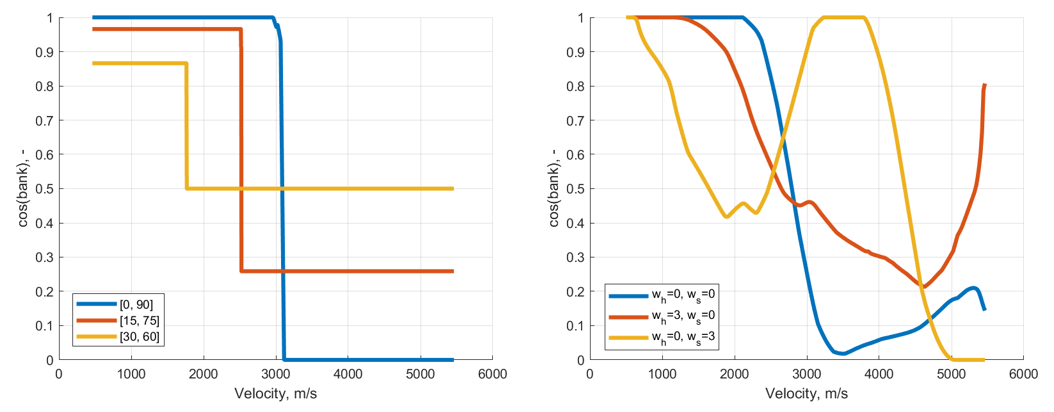
\includegraphics[width=1\textwidth]{ddp/comparison_controls}
	\caption{The profiles from deterministic optimal control (left) exhibit the well known bang-bang structure of altitude optimal trajectories. In comparison, the robust control histories (right) exhibit significantly behavior depending on the weights applied. Note that a significant amount of saturation of the reference control still exists in each of the robust reference designs.}
	\label{fig_control_comparison}
\end{figure}
Figure~\ref{fig_control_comparison} shows the resulting control profiles for the six cases. The altitude-optimal controls resulting from standard optimal control exhibit the well known bang-bang profile while the robust optimal control profiles are quite varied depending on the weights selected. For pure mean optimization, the result is somewhat similar to the bang-bang profiles, but retains margin at high velocities and has a slower transition to the lift up ($u=1$) orientation. An interesting feature of the robust profiles is that saturation still occurs at some velocities. This suggests that the optimal amount of margin is a quantity that varies along the trajectory, which implies using a fixed margin will produce inferior results.
% Methods that incorporate chance constraints on the control in order to reduce saturation cannot accomplish this.

For each case, a Monte Carlo simulation with 2000 sample trajectories is conducted to evaluate the performance of each reference. The samples are drawn using Latin Hypercube sampling. The results are summarized in Tables~\ref{table_deterministic}-\ref{table_robust}. Case 1 preserves no margin at all, and as a result has the highest nominal terminal altitude of the three cases. This translates into the highest mean altitude of the three cases, despite the lack of margin. However, the lack of margin causes poor range control performance in dispersed trajectories, leading to unacceptably large mean and 3$\sigma$ range errors. As the amount of control margin increases in Cases 2 and 3, both the mean and 3$\sigma$ range errors drop dramatically while the mean altitude also decreases. The 3$\sigma$-low altitudes display non-monotonic behavior with respect to bank margin because the mean altitude loss may or may not be offset by the reduction in altitude deviation. This is true for Case 2, which has a higher 3$\sigma$-low altitude relative to Case 1. In Case 3, the drop in mean altitude is greater than the drop in the 3$\sigma$-low altitude because the altitude deviation has decreased further. 

Case 4 ($ w_h=w_s=0 $) optimizes the mean altitude with knowledge of the problem uncertainty and guidance gains. The mean altitude is 50 m lower than Case 1 because the UT overestimated the mean. However, this difference is quite small, and the performance is more robust because the 3$\sigma$-low altitude is higher and the 3$\sigma$ range error is smaller. Case 5 ($ w_h=3,w_s=0 $) adds additional weight to the altitude standard deviations, which resulted in a 500 meter increase to the 3$\sigma$-low altitude despite a 300 meter drop in mean altitude relative to Case 4. Case 5 has the highest 3$\sigma$-low altitude of the six cases, with more than a kilometer increase over the best of the three profiles designed without incorporating uncertainty. Case 6 ($ w_h=0, w_s=3$) places no weight on altitude standard deviation, but weights range errors heavily, and produces a dramatic decrease in 3$\sigma$ range errors as a result. It has the lowest range error of the six cases, and compared to the large margins of case 3, still produces a higher 3$\sigma$-low altitude.

This demonstrates the applicability of optimal control under uncertainty to designing robust reference trajectories. Additionally, the flexibility of the weights allows the trajectory designer to trade between range errors and altitude performance to the extent that the reference trajectory can alter closed-loop performance. 
\begin{table}[h!]
	\centering
	\caption{Monte Carlo statistics for cases 1-3, designed using optimal control and fixed bank margins.}
	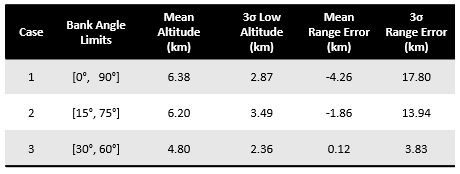
\includegraphics[width=0.65\textwidth]{ddp/table_deterministic}
	\label{table_deterministic}
\end{table}
\begin{table}[h!]
	\centering
	\caption{The Monte Carlo statistics for cases 4-6, designed using the proposed method.}
	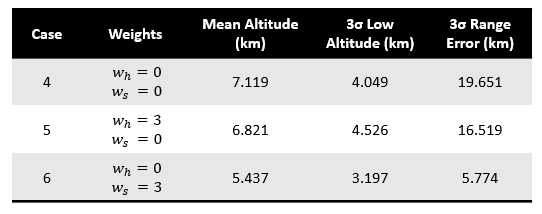
\includegraphics[width=0.65\textwidth]{ddp/table_robust} %
	\label{table_robust}
\end{table}
%Figures~\ref{fig_robust_alt}-\ref{fig_robust_range} show the estimated $3\sigma$ deviations around the mean as well as the sigma point trajectories for scenario 1.
%\begin{figure}[h!]
%	\centering
%	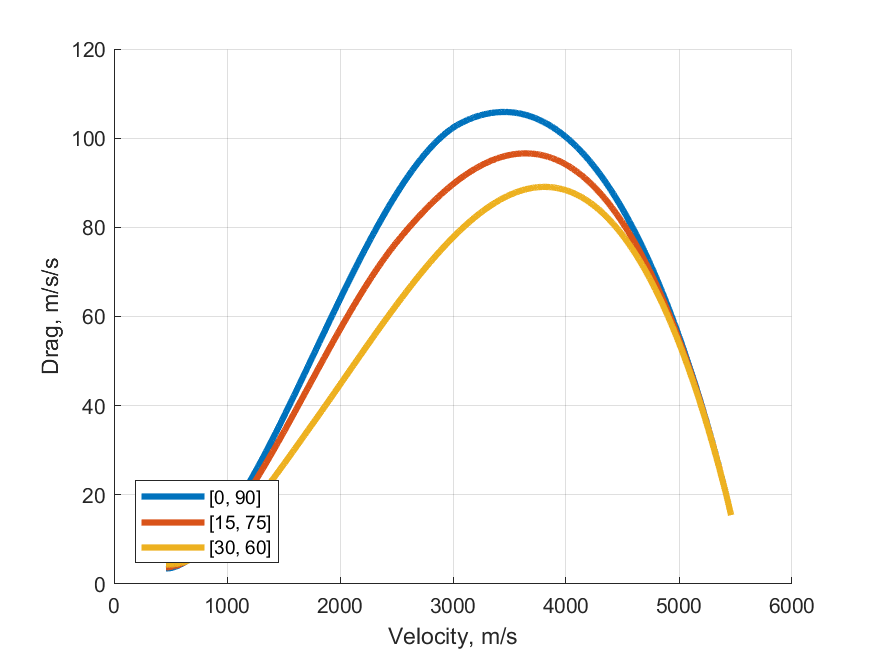
\includegraphics[width=1\textwidth]{ddp/matlab/NominalDrag}
%	\caption{Reference drag profile for each of the four scenarios in Table~\ref{table_comparison}.}
%	\label{fig_drag}
%\end{figure}
%\begin{figure}[h!]
%	\centering
%	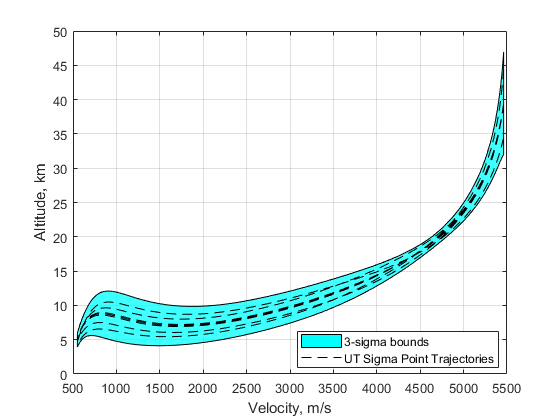
\includegraphics[width=1\textwidth]{ddp/matlab/RobustTrajAlt}
%	\caption{Dispersed altitude performance for scenario 1.}
%	\label{fig_robust_alt}
%\end{figure}
%\begin{figure}[h!]
%	\centering
%	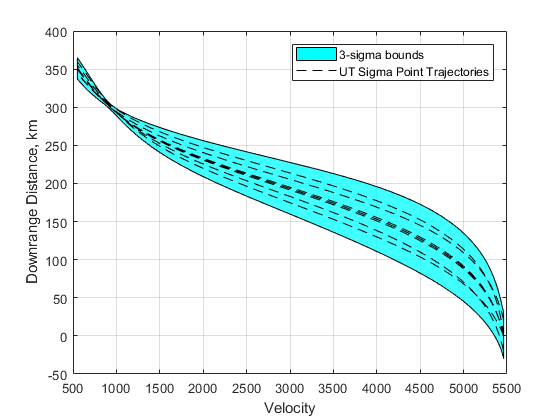
\includegraphics[width=1\textwidth]{ddp/matlab/RobustTrajRange}
%	\caption{Dispersed range performance for scenario 1.}
%	\label{fig_robust_range}
%\end{figure}


\subsection*{Standard Deviation Weighting Study}
\begin{figure}[h!]
	\centering
	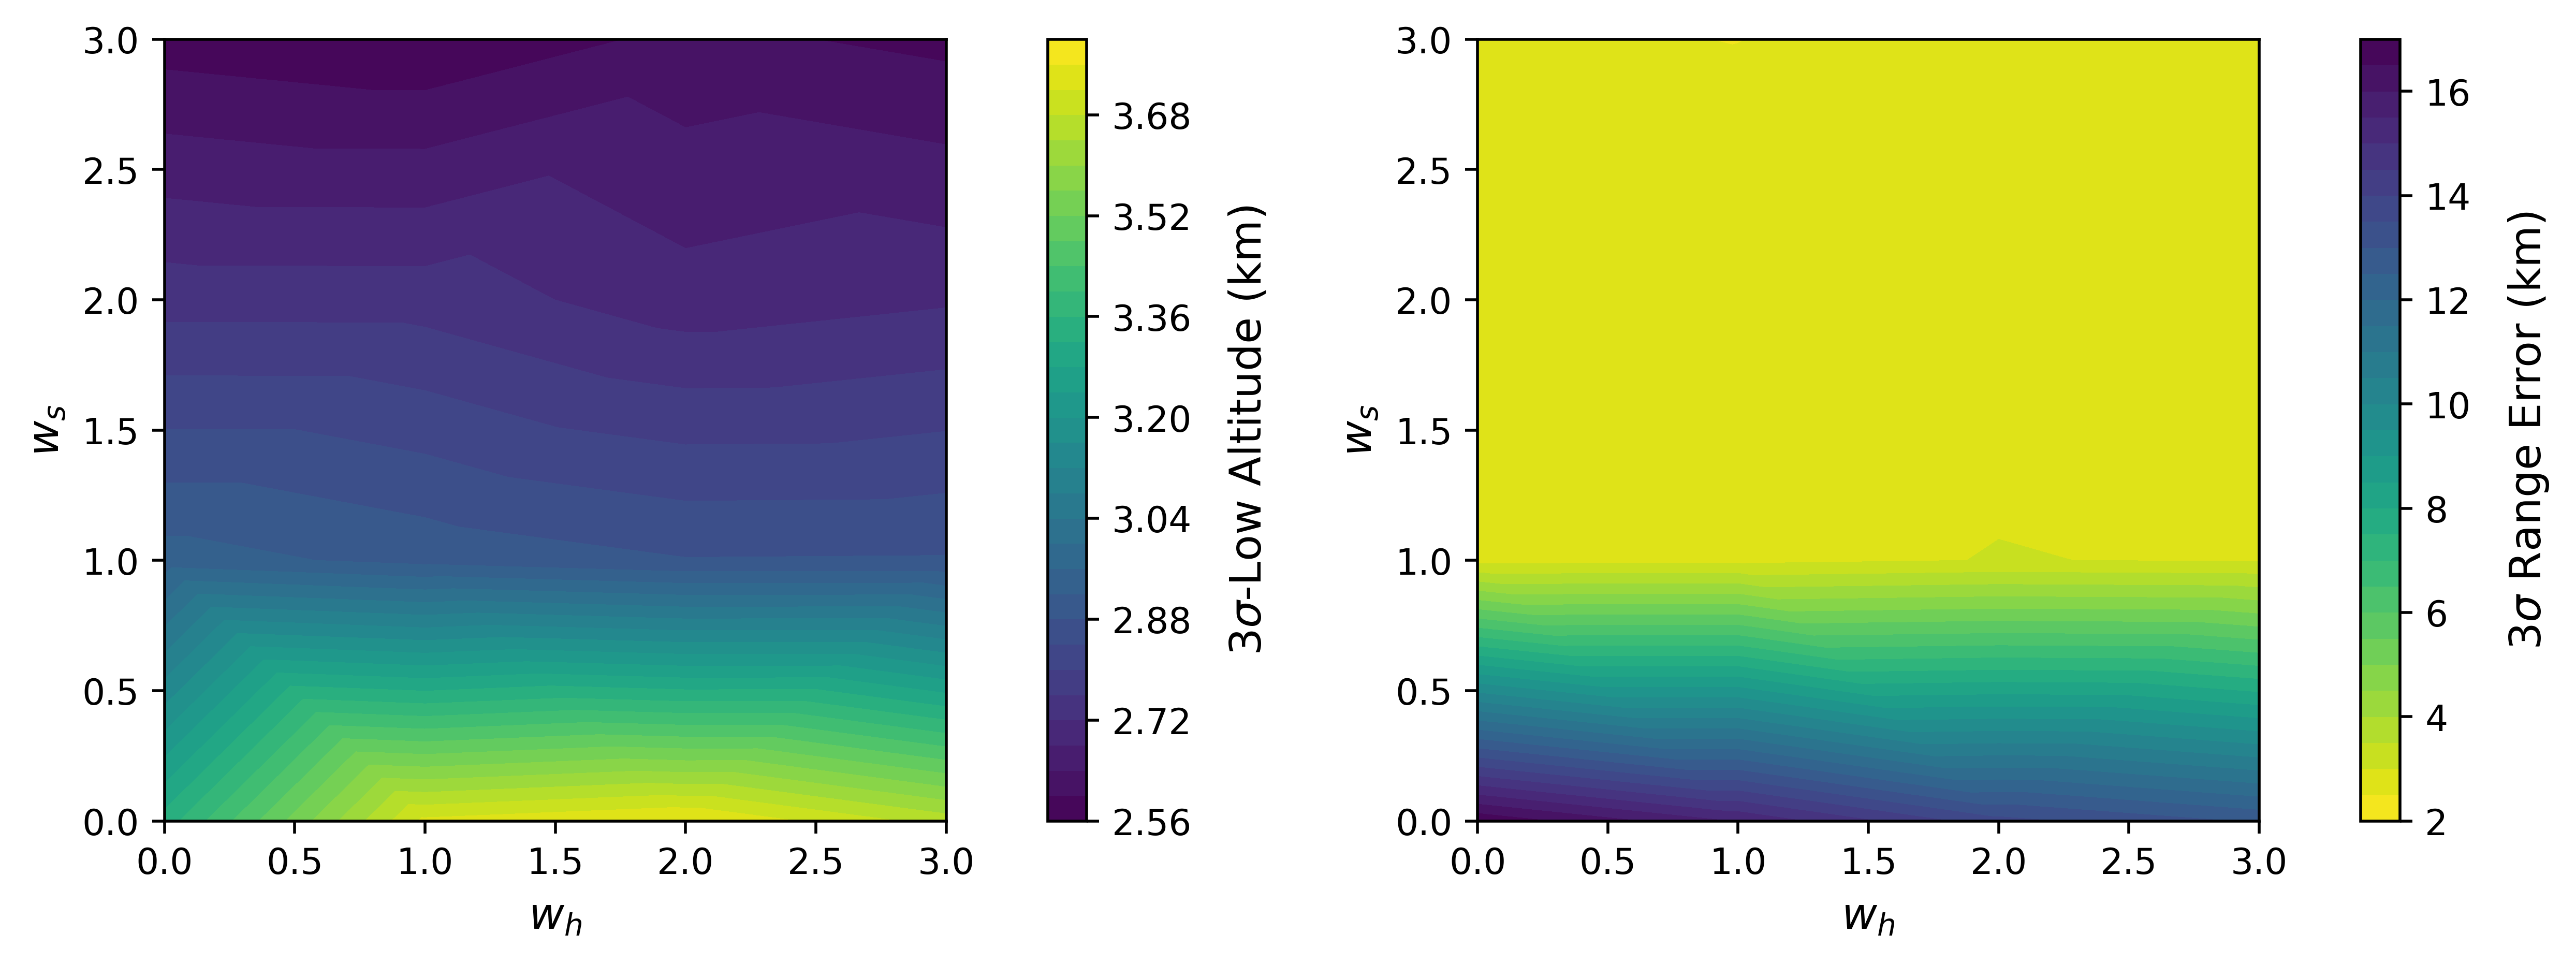
\includegraphics[width=1\textwidth]{ddp/python/WeightSweepMC}
	\caption{Contours of the Monte Carlo 3$\sigma$ low altitude (left) and 3$\sigma$ downrange distance error (right) as a function of the weights $w_h$ and $w_s$.}
	\label{fig_weight_sweep}
\end{figure}
%TODO: Double check these numbers, they may have changed 
From the previous subsection it is evident there exists a design space where weights on deviations produce superior results to simply optimizing the mean altitude when tail behavior of the distribution is important. This section investigates the extent to which weighting the standard deviations can alter the trajectory performance. The optimal control problem is solved for a variety of weights. The results are summarized in Fig.~\ref{fig_weight_sweep}. Again the advantages of weighting the standard deviations compared with optimizing only the mean are made clear. Comparing $w_h=w_s=0$ with, e.g., $w_h=1,\,w_s = 1$ demonstrates that a 50\% reduction in the standard deviation of downrange distance can be obtained with no loss in the low end of the terminal altitude distribution. Additionally, we can numerically determine the trade between terminal altitude and downrange robustness. The minimum downrange standard deviation achieved ($w_h=1,w_s=3$) was 0.7 km, an 85\% reduction from the mean optimization with $\sigma_s(v_f)=5.1$ km. These trajectories show clear improvements with no change to the guidance gains - simply a different reference trajectory is used to improve the results. The downrange distance shows only small improvement for weights $w_s>1$, but the low altitude continues to drop as this weight is increased. Thus, a compromise such as $w_h=w_s=1$ strikes a good balance between the two objectives. 

These results also show some inaccuracy due to using the unscented transform. The 3$\sigma$-low altitude should be maximized when the objective function is exactly this quantity, i.e., $w_h=3,\,w_s=0$, but due to small estimation errors this is not the case, and the highest 3$\sigma$-low altitude is achieved with $w_h=2,\,w_s=0$. Similarly, the 3$\sigma$ range error is not minimized when $w_h=0,\,w_s=3$, but instead $w_h=1,\,w_s=3$. However, the difference in each of these cases is quite small. This issue is related to that fact that a constant UT scaling parameter $\alpha=15$ is used in all computations. Our experience with the numerical results suggests that the optimal value of $\alpha$ depends on the weights selected, and larger weights should use a higher $\alpha$. 
%Nevertheless, the solutions at all weight values are acceptable
%This also highlights the power of the approach as a design tool. If, for example, the $3\sigma$-low terminal altitude is not sufficient for any values of $w_h,\,w_s$, then some aspect of the mission must be reconsidered: increase the terminal velocity, increase the vehicle $L/D$, decrease ballistic coefficient, etc. If a $3\sigma$-low altitude limit is known, then only points that satisfy this limit are considered, and the point with the lowest downrange error may be selected. 

These results used constant feedback gains, so it is likely that methods of generating gains that vary along the trajectory, such as the Linear-Quadratic Regulator, Apollo influence coefficients \cite{Apollo}, or joint optimization of the feedback gains in the optimal control problem, could produce even greater synergistic improvements to the trajectory design. 

\subsection*{Monte Carlo Example}
\begin{table}[h!]
	\centering
	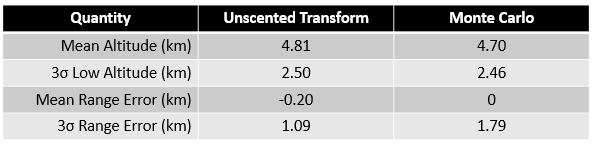
\includegraphics[width=0.75\textwidth]{ddp/table_mc}
	\caption{Summary of the statistics from the Unscented Transform and Monte Carlo}
	\label{table_mc}
\end{table}
\begin{figure}[h!]
	\centering
	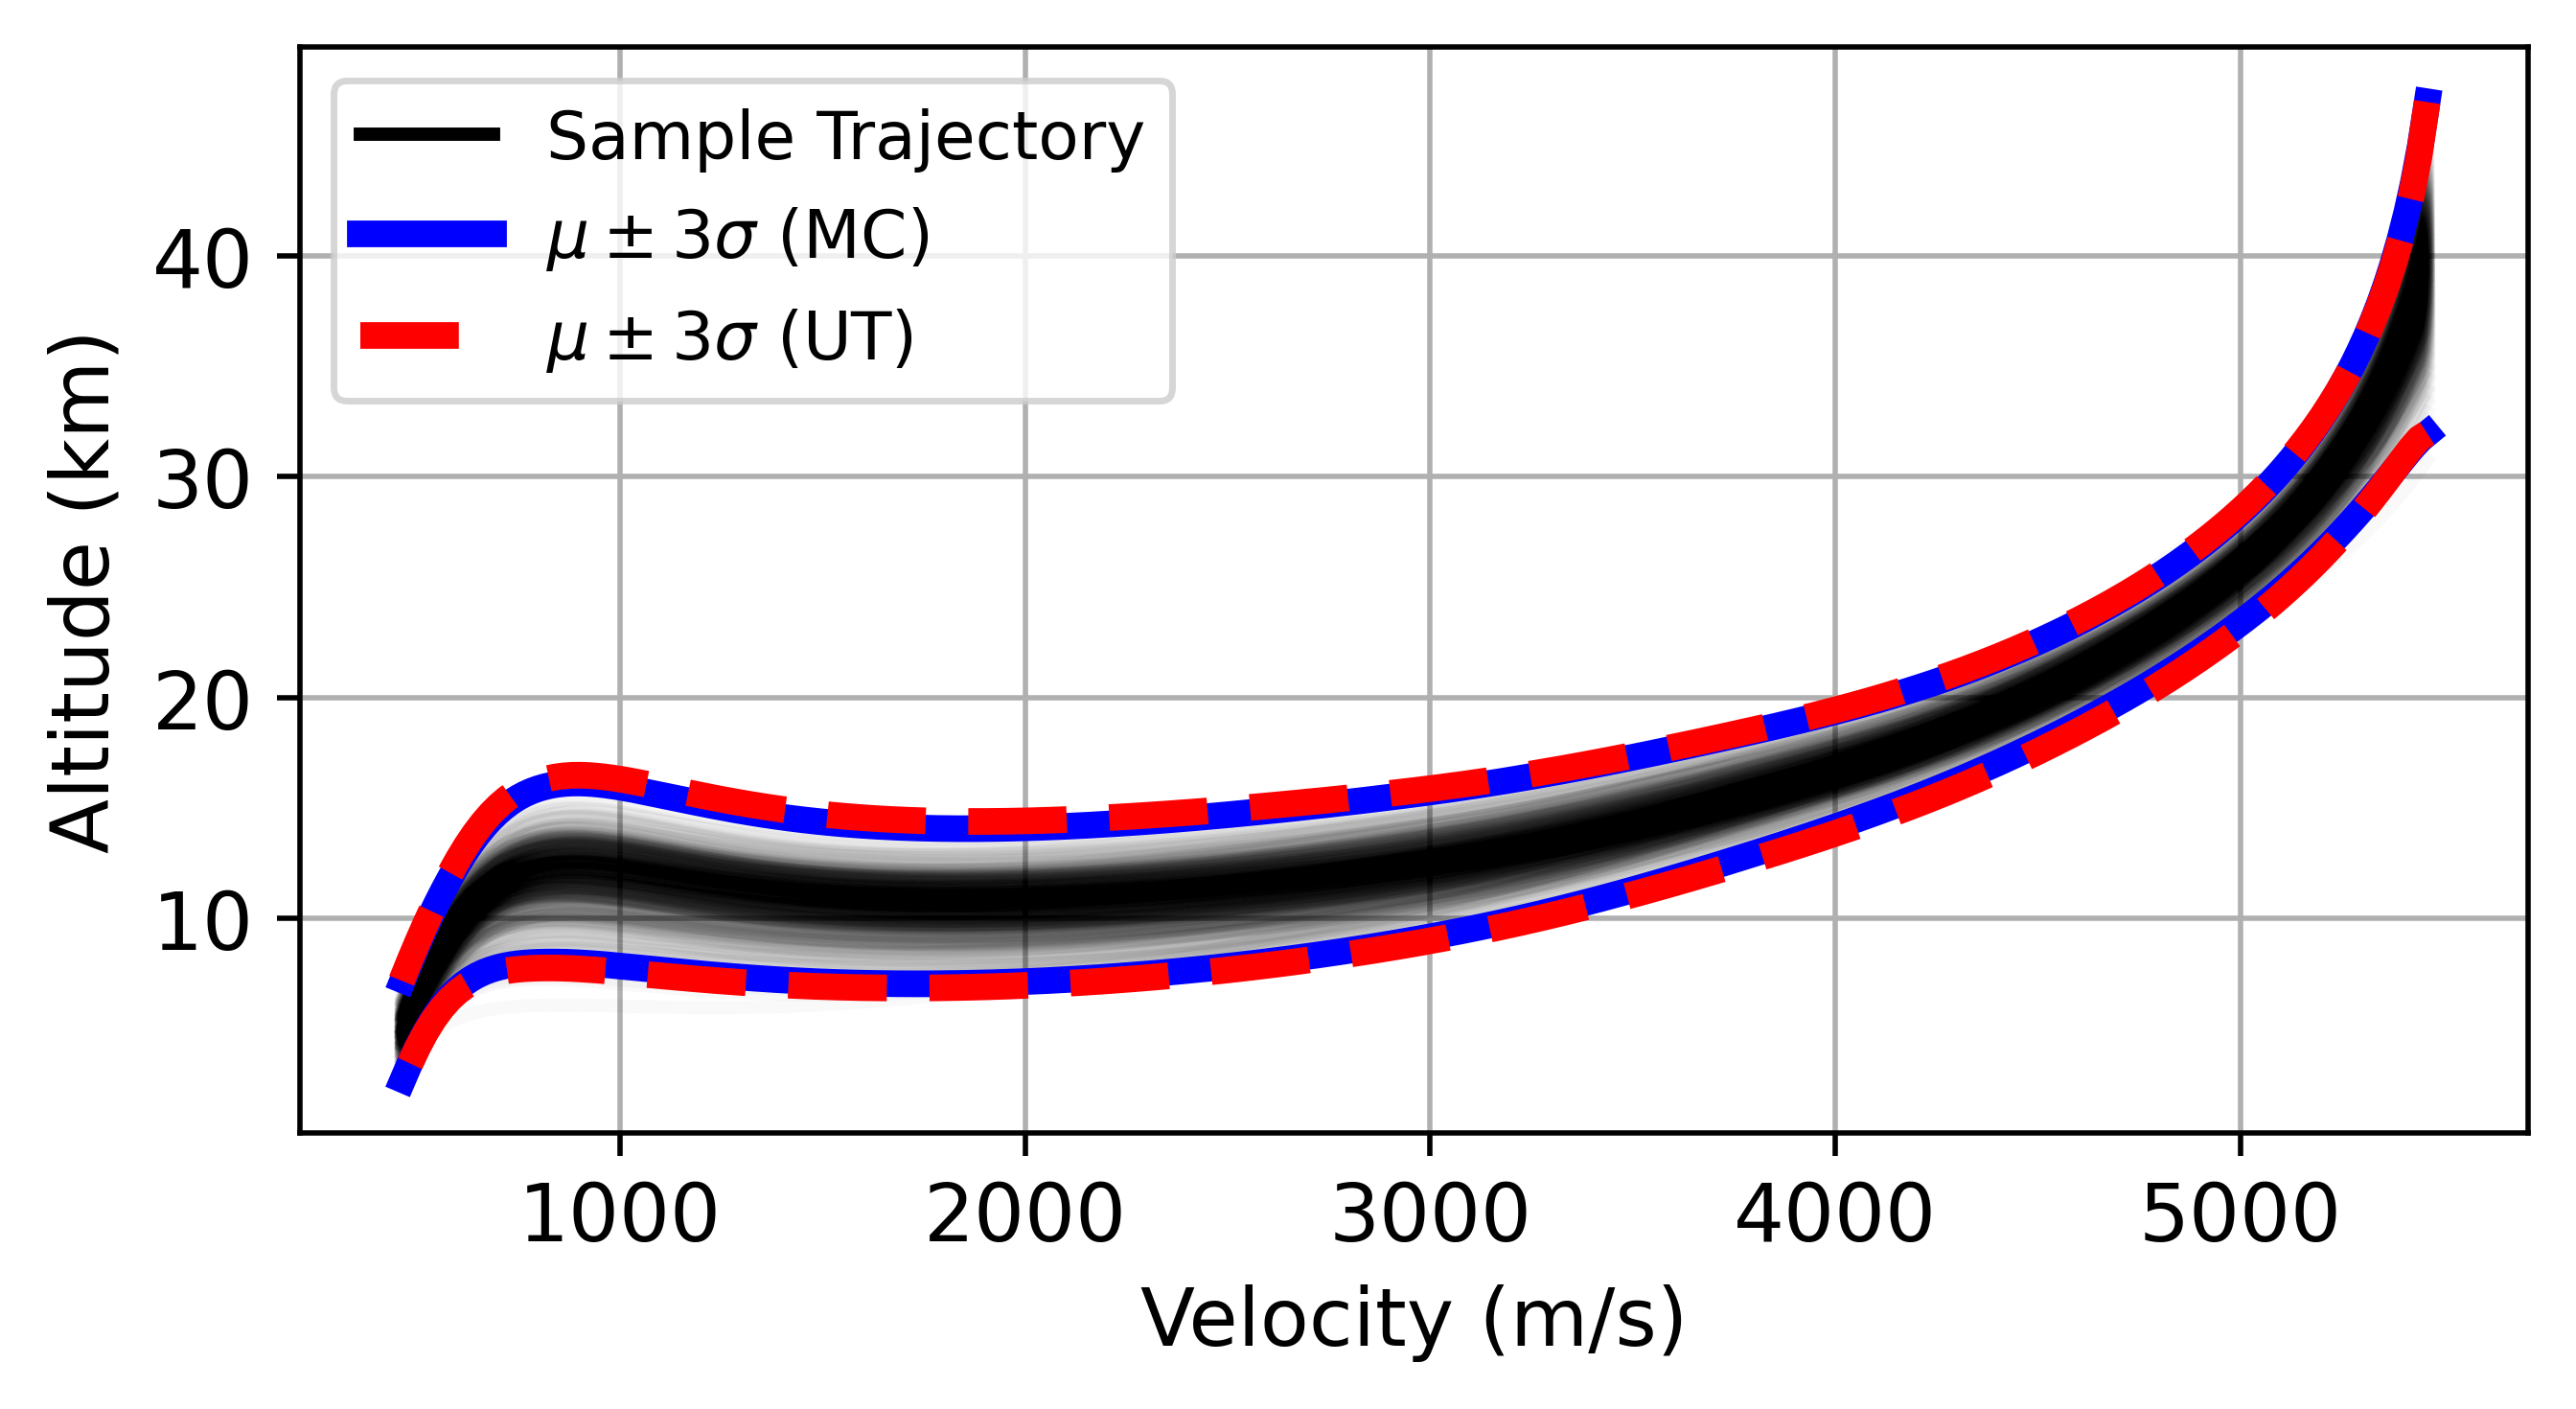
\includegraphics[width=0.75\textwidth]{ddp/python/Altitude}
	\caption{The altitude versus velocity Monte Carlo results and UT-estimated bounds. The 3$ \sigma $-low altitude is 2.5 km.}
	\label{fig_mc_alt}
\end{figure}
\begin{figure}[h!]
	\centering
	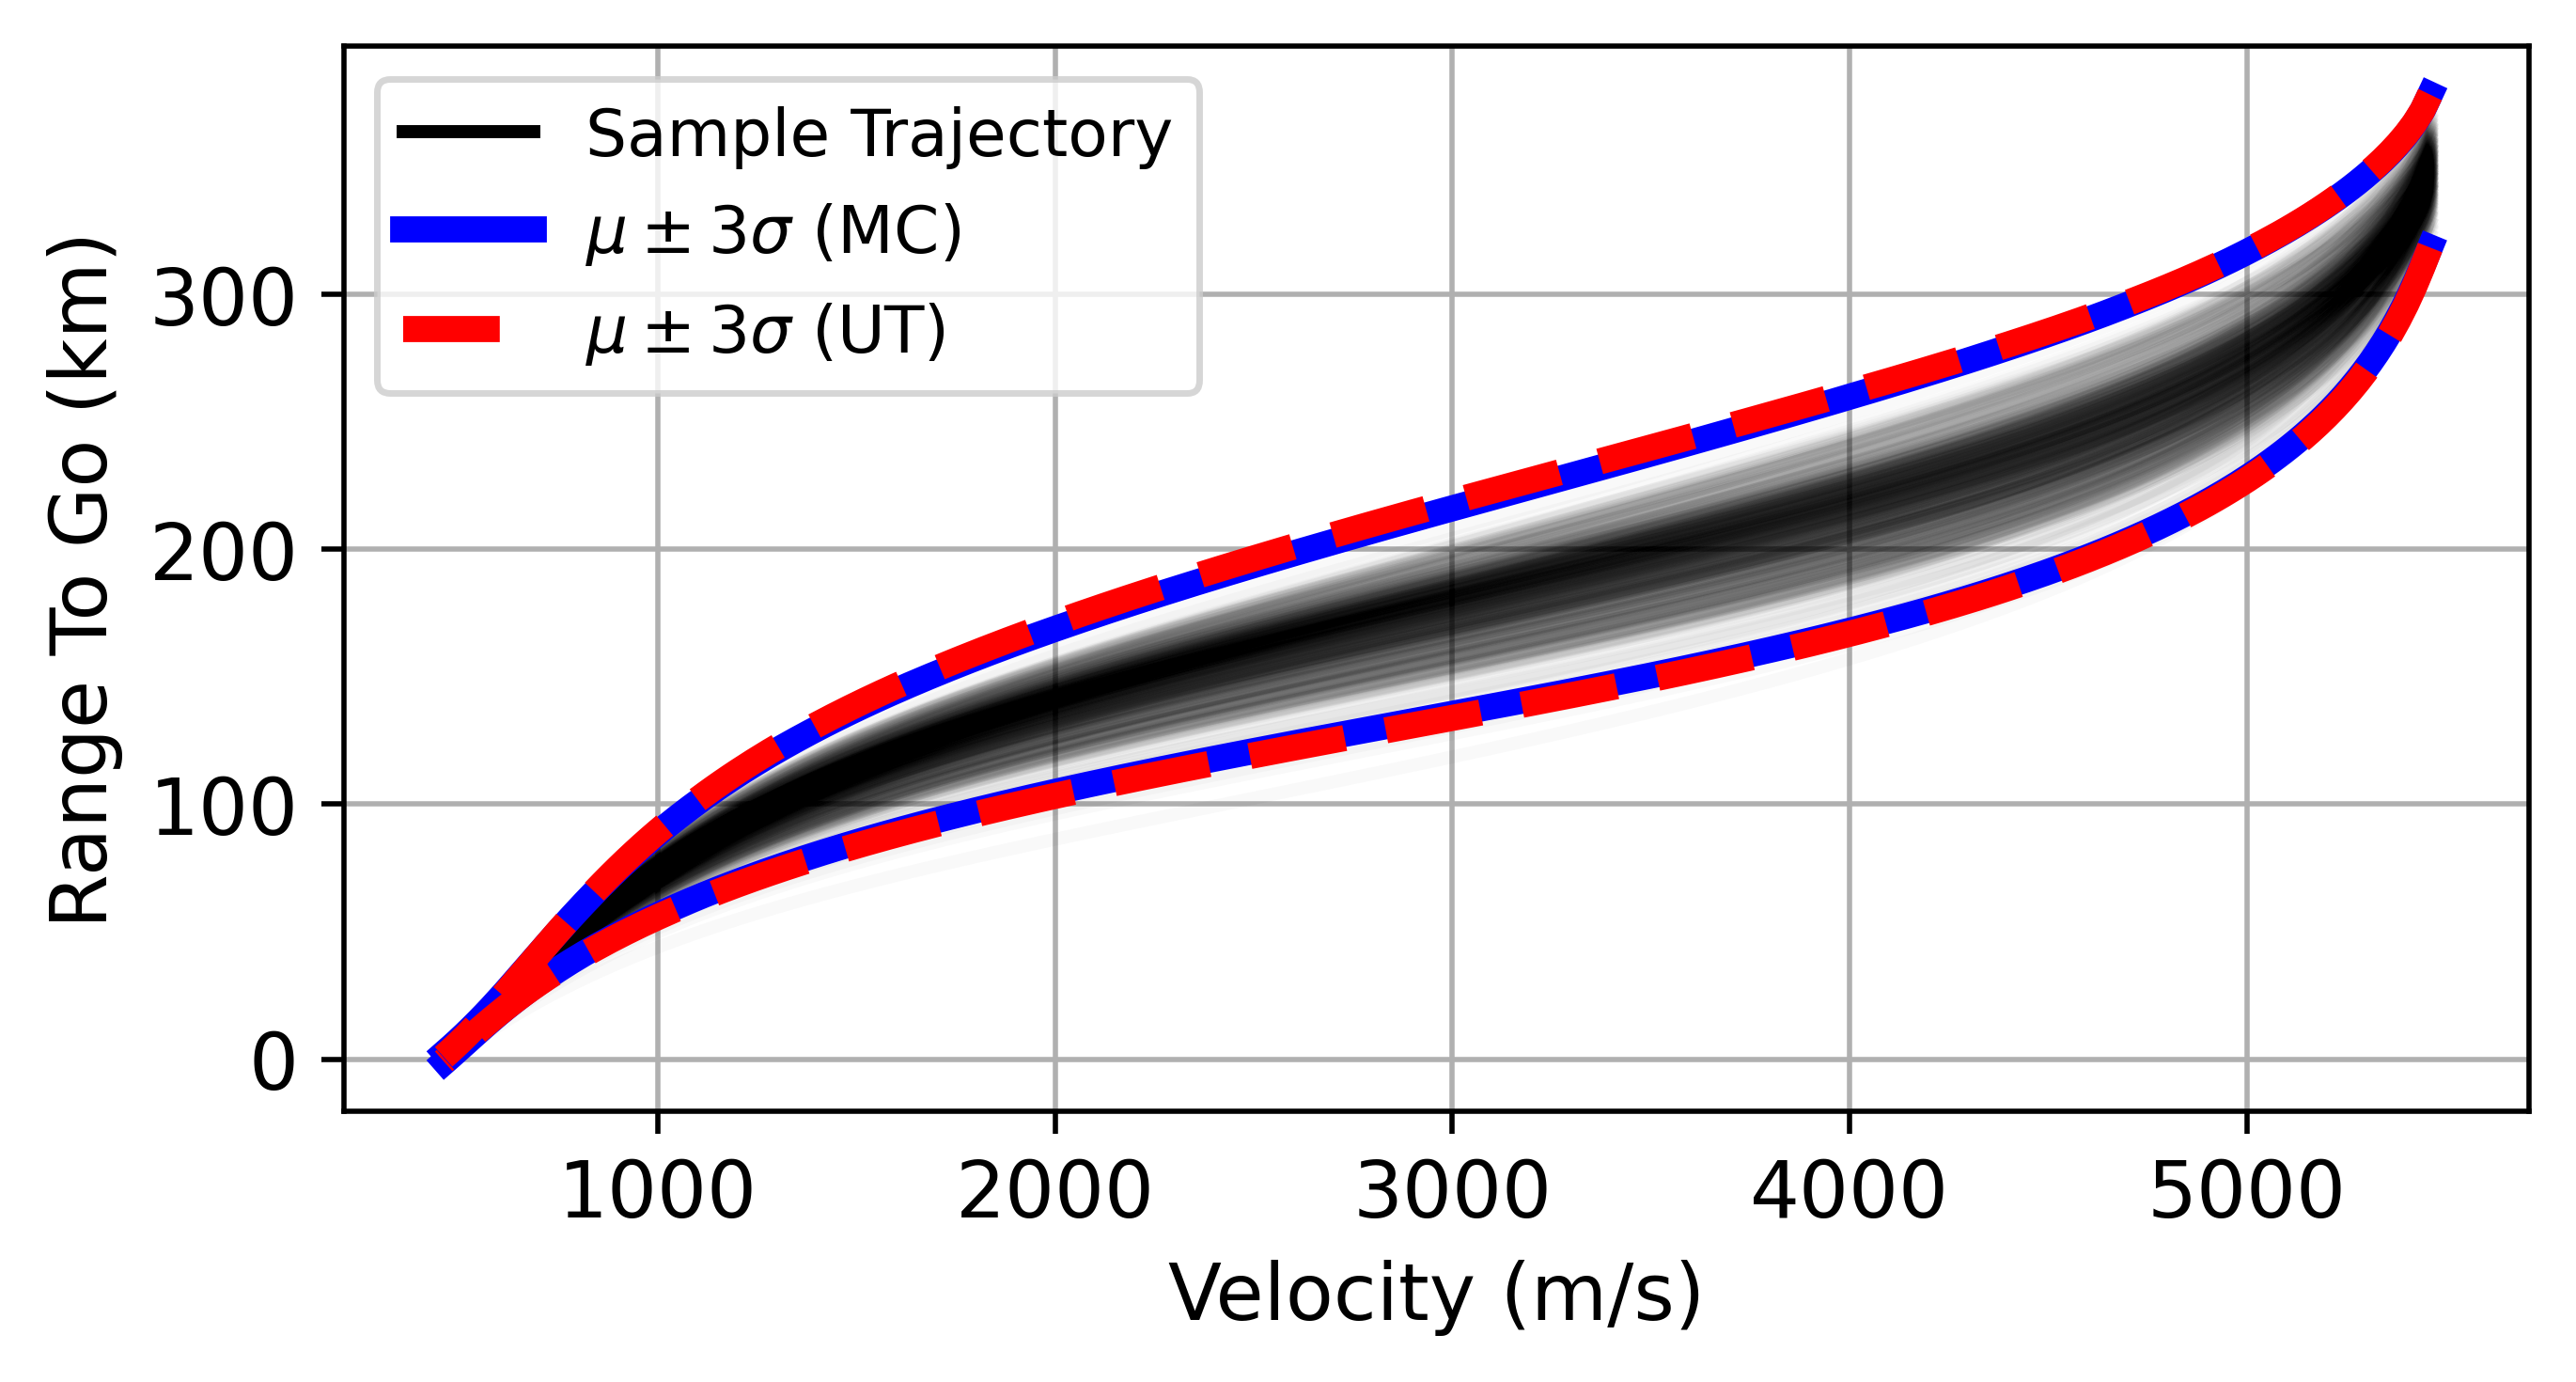
\includegraphics[width=0.75\textwidth]{ddp/python/Range}
	\caption{The downrange versus velocity Monte Carlo results and UT-estimated bounds. The terminal 3$ \sigma $ range error is 1.8 km.}
	\label{fig_mc_range}
\end{figure}
\begin{figure}[h!]
	\centering
	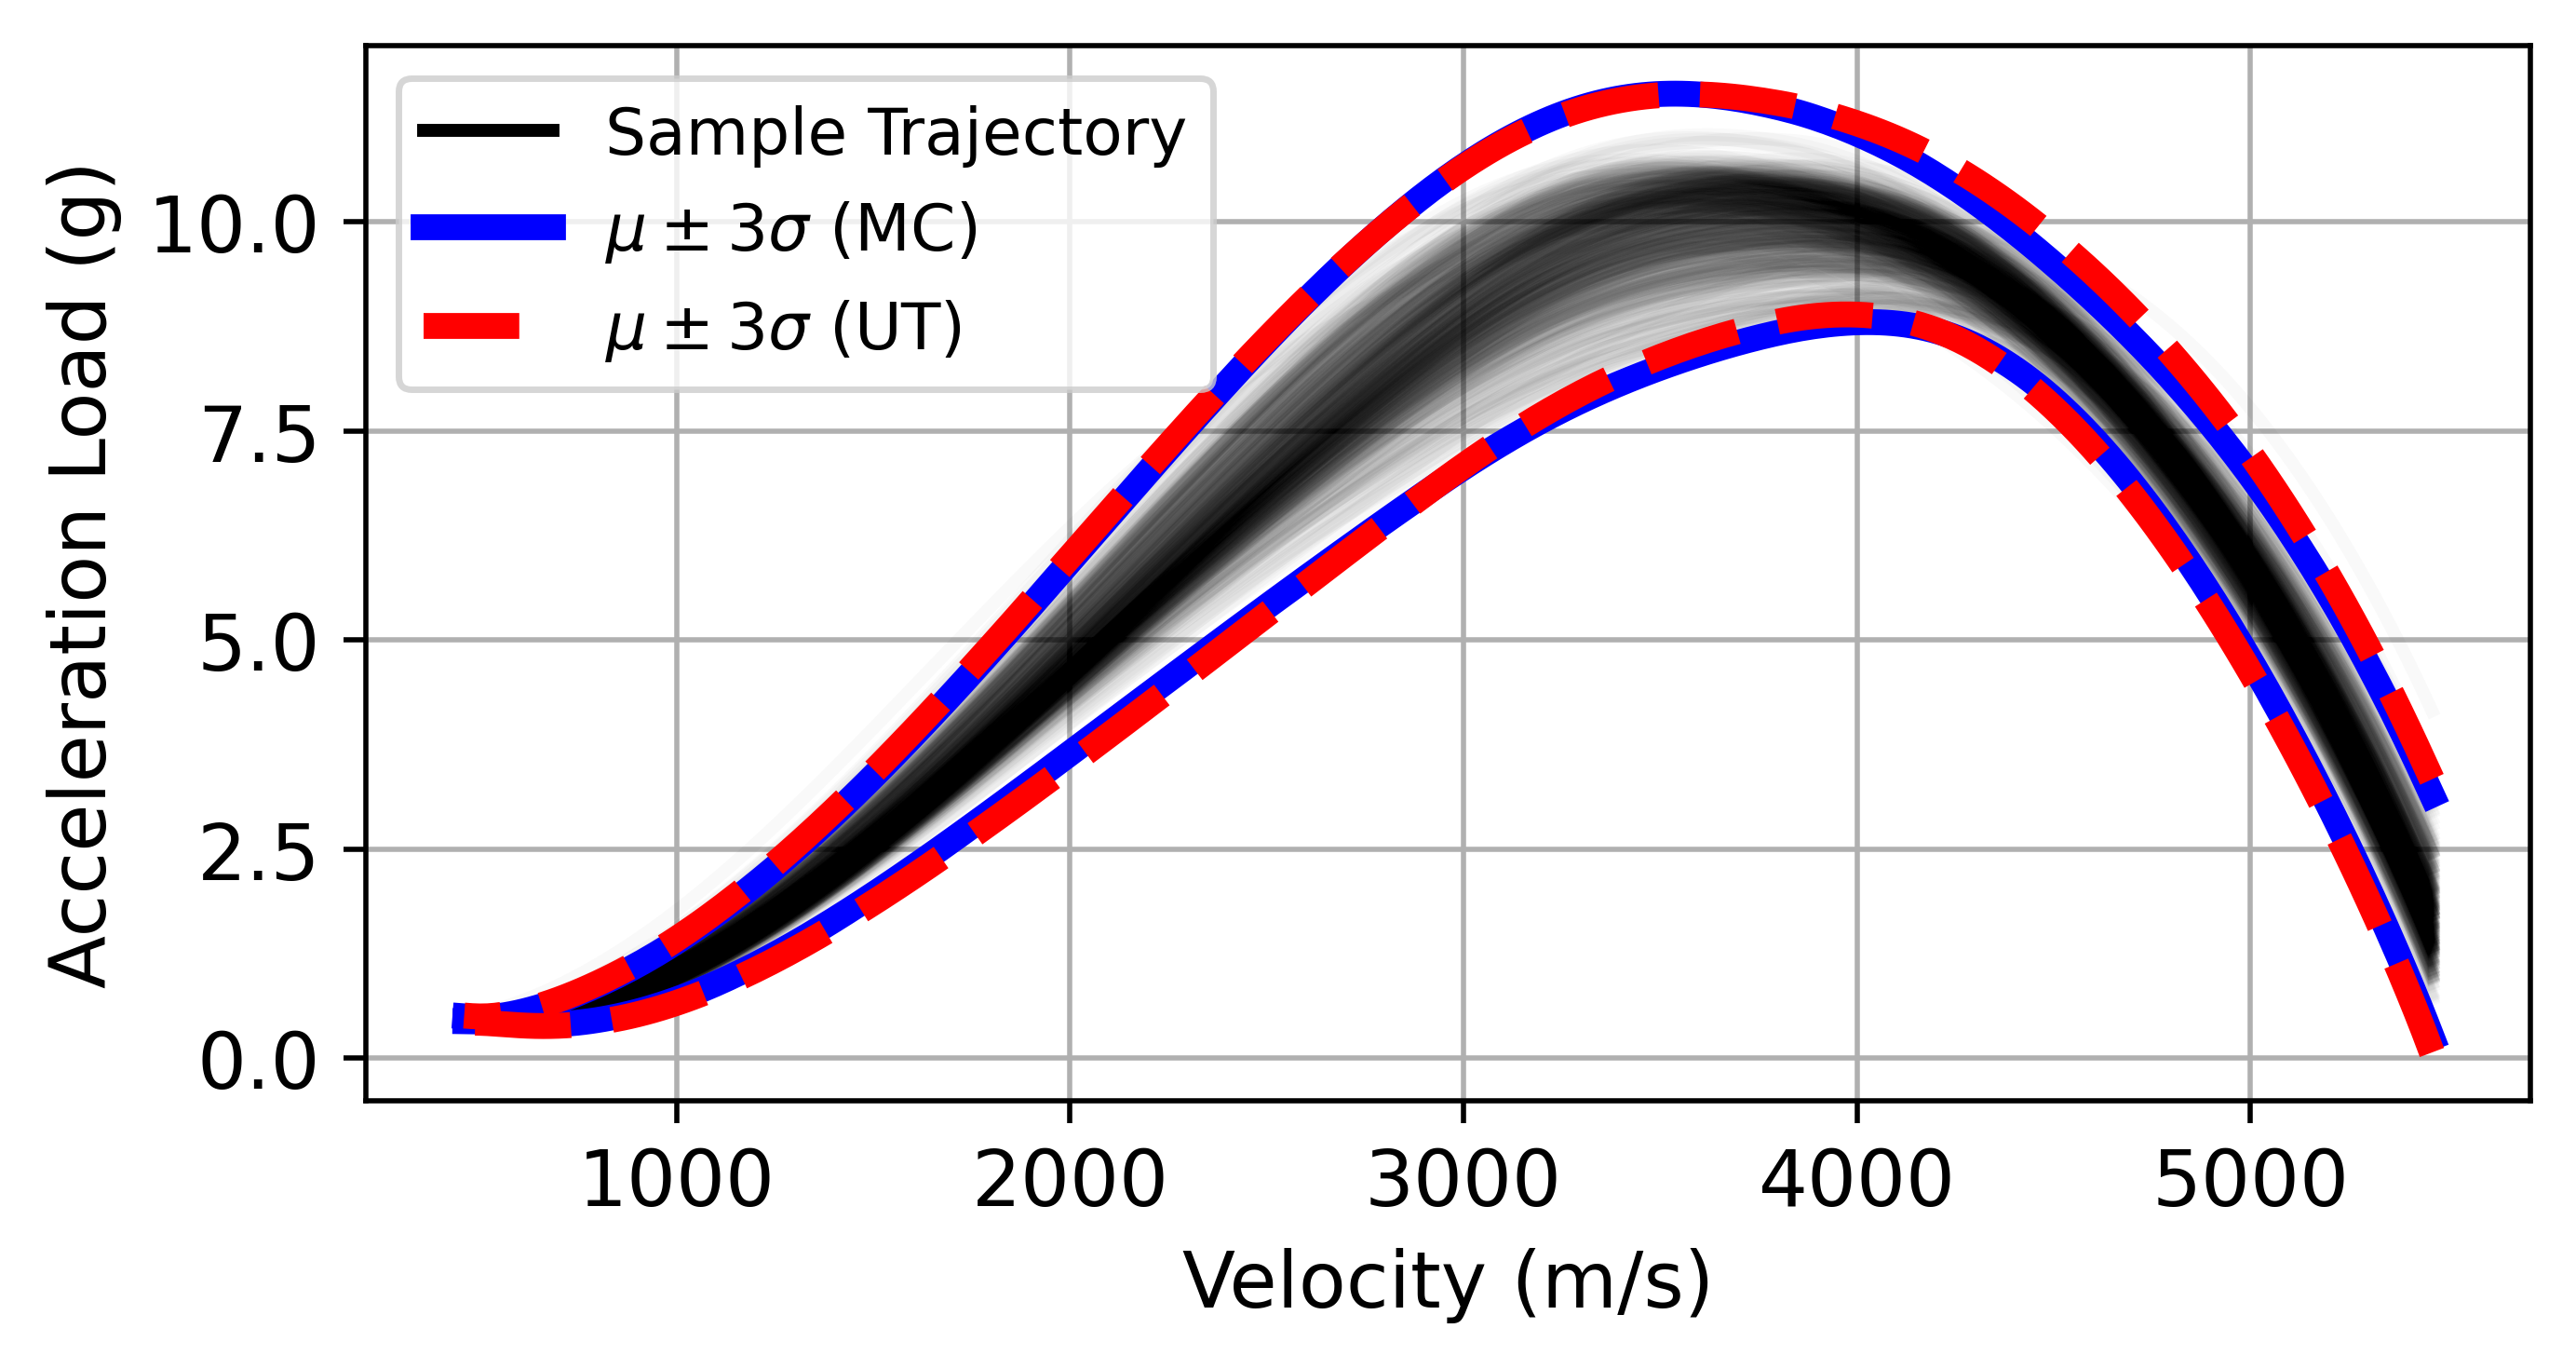
\includegraphics[width=0.75\textwidth]{ddp/python/Acceleration}
	\caption{}
	\label{fig_mc_accel}
\end{figure}
\begin{figure}[h!]
	\centering
	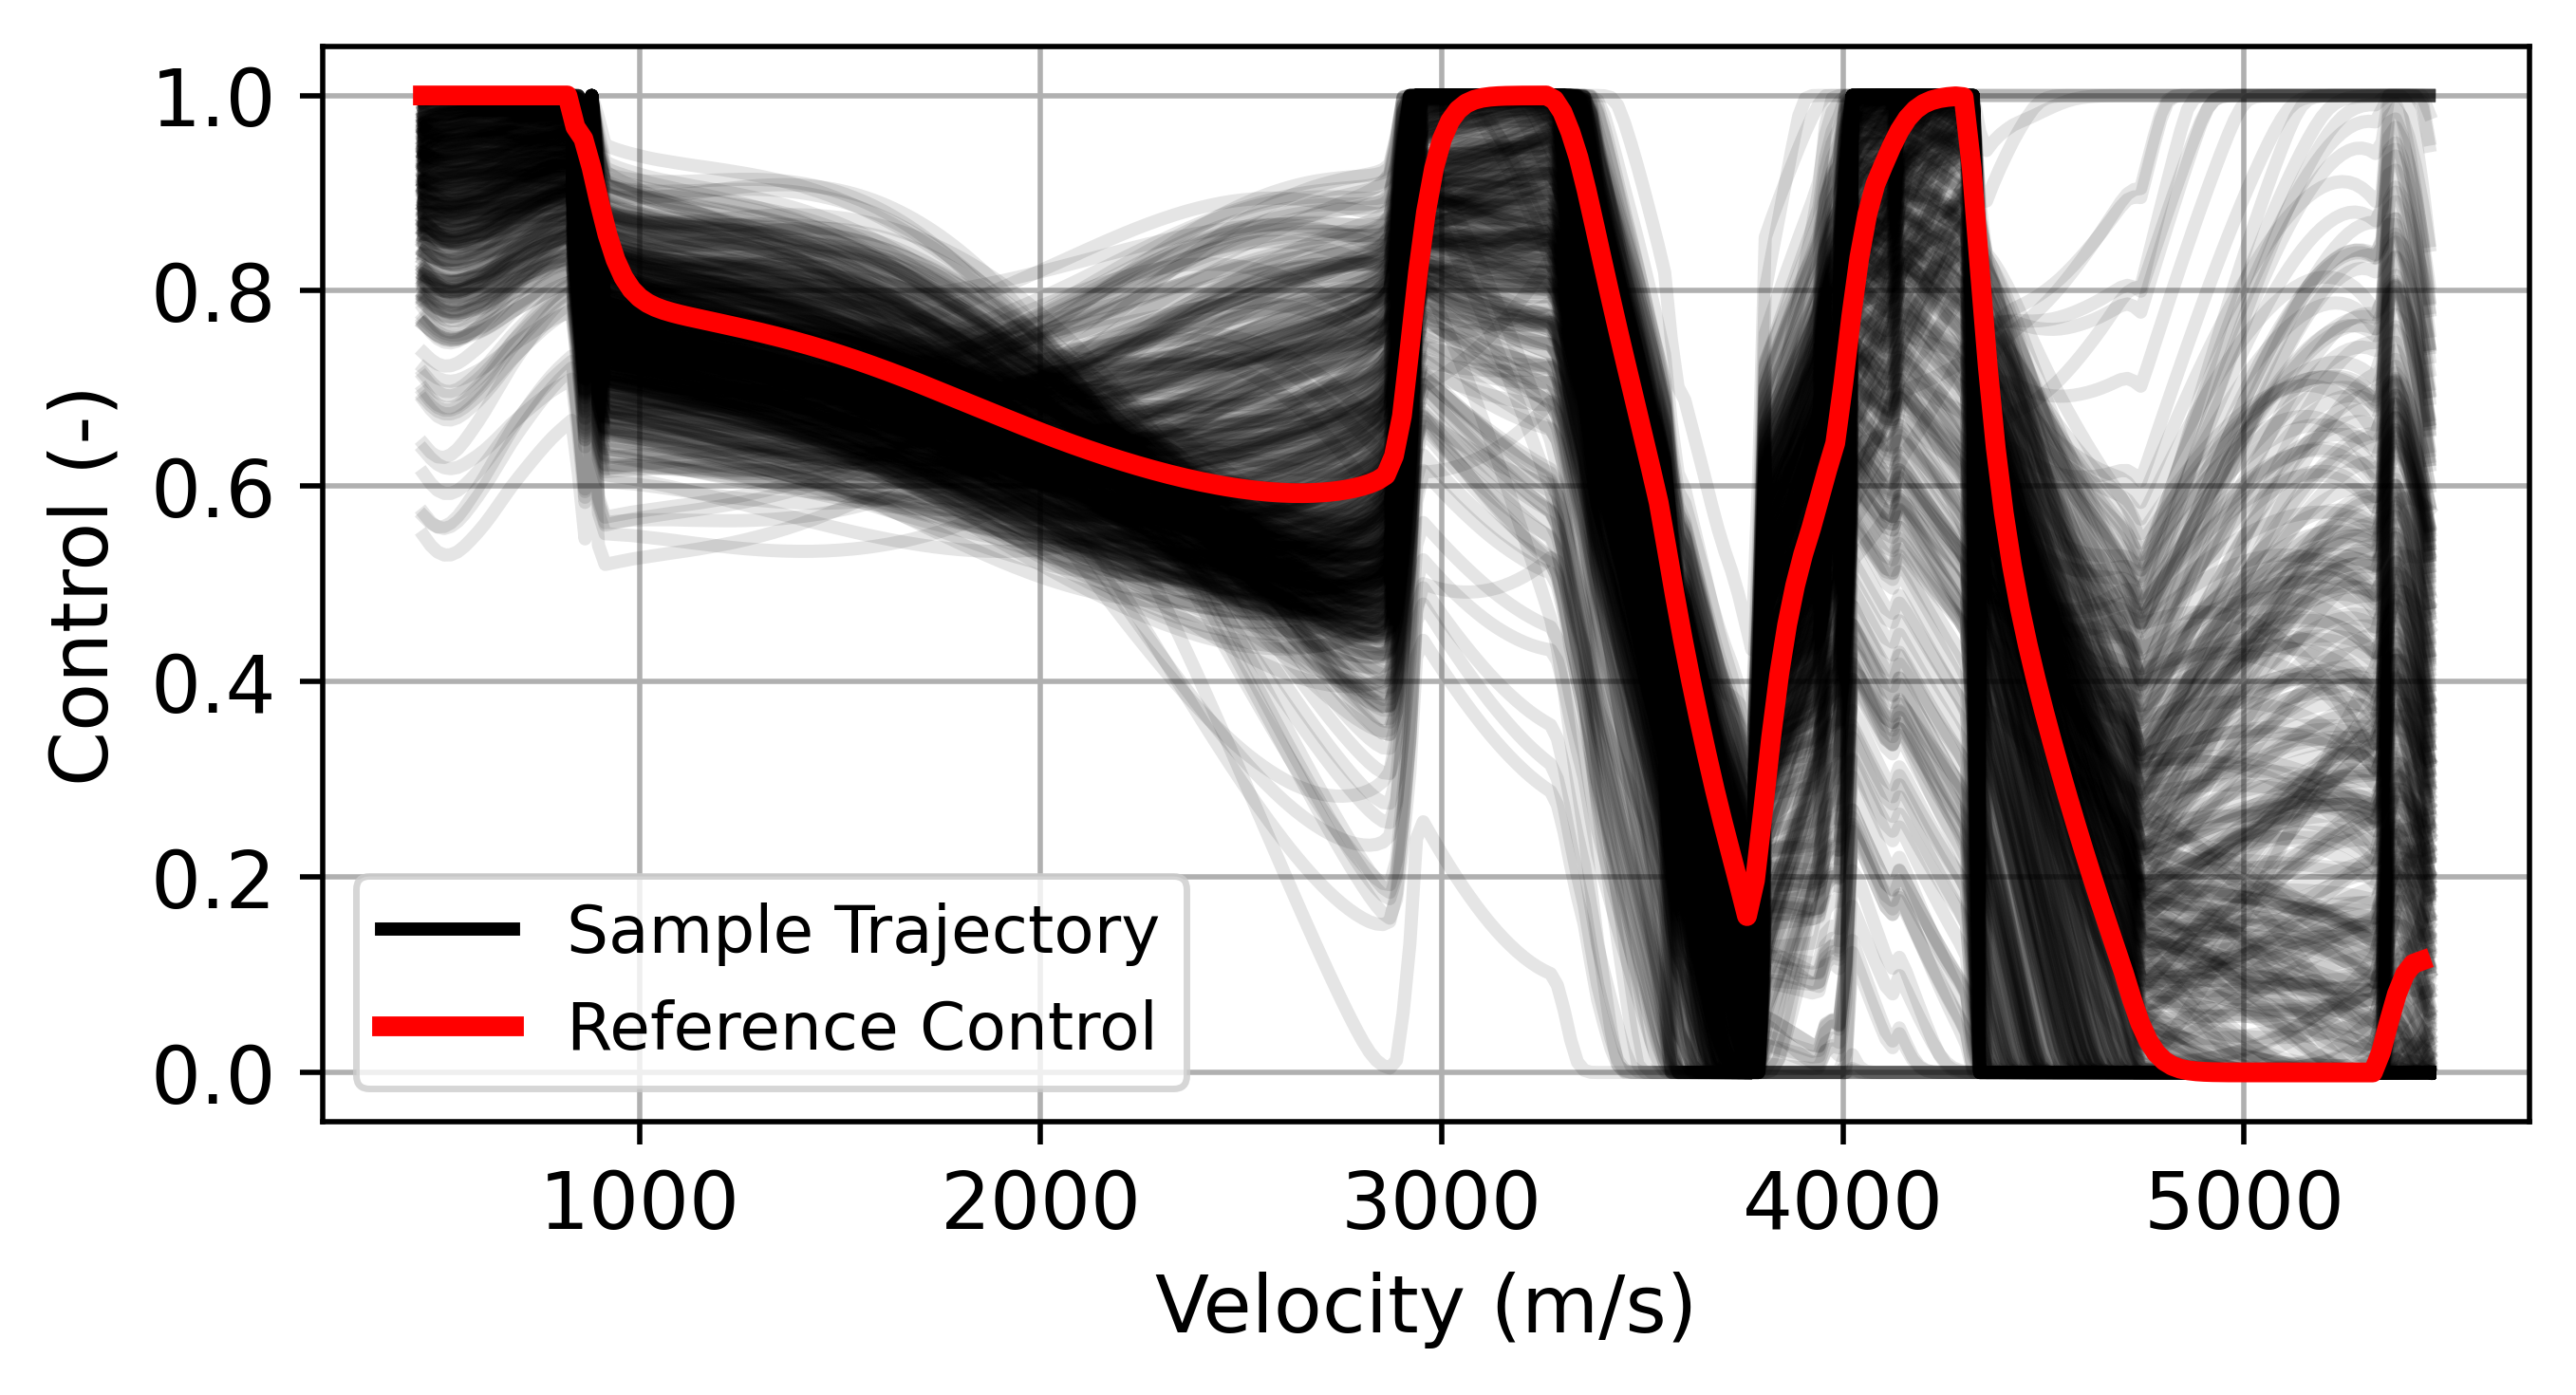
\includegraphics[width=0.75\textwidth]{ddp/python/Control}
	\caption{The reference control and 500 sample trajectories.}
	\label{fig_mc_control}
\end{figure}
The previous subsections looked at broader trends when using the proposed method to design reference trajectories. This subsection will focus on a single solution and present more detailed Monte Carlo results and discussion. Since both objectives are important and a compromise must be met, we select the weights $w_h=w_s=1$. A Monte Carlo simulation was conducted with 8000 samples in order generate precise statistics for comparison with the unscented transform. The feedback gains were again constants, but for this case they were reoptimized to minimize range errors after finding the optimal reference control with the previous gains. The result was $[k_D, k_{\gamma}, k_s] = [0.058, -0.021, -0.005]$, and a reduction in the 3$\sigma$ range error from 2.5 km to 1.8 km.
Table~\ref{table_mc} compares statistics estimated with the unscented transform and Monte Carlo simulation. Relative to the Monte Carlo results, the UT overestimates the mean altitude by 100 m, the low altitude by 40 m, and underestimates the range error by 700 m or nearly 40\%. Nevertheless, the reference trajectory and constant gains are still quite effective with the Monte Carlo range error under 2 km. Because the mean trajectory is used as the reference, the UT-estimated mean error is always zero. 
Figures~\ref{fig_mc_alt}-\ref{fig_mc_accel} show 500 sample trajectories as well as the Monte Carlo estimated 3$\sigma$ bounds, and the UT-estimated 3$\sigma$ bounds for comparison. Figure~\ref{fig_mc_alt} shows that lofting at low velocities is a key feature of the trajectories used to raise the terminal altitude. Figure~\ref{fig_mc_accel} shows the acceleration loads which never exceed 12g.
Contrary to claims that range control is not effective at low velocities \cite{MSL_EDL2}, Fig.~\ref{fig_mc_range} shows the convergence of the 3$\sigma$ range errors from 25 km at $ v=1100 $ m/s to less than 2 km at the $v=460$ m/s. Each of these figures demonstrates that the UT estimated statistics are quite close to the Monte Carlo results. Figure~\ref{fig_mc_control} shows the reference control as well as the sample controls for the same 500 trajectory subset. The reference control resembles min-max profiles at high velocities before transitioning gradually to a full lift up orientation. Many of the samples have saturated controls over significant portions of the trajectory.  

\section*{Conclusion}
%Although a conclusion may review the main points of the paper, it must not replicate the abstract. A conclusion
%might elaborate on the importance of the work or suggest applications and extensions. Do not cite references in the
%conclusion. Note that the conclusion section is the last section of the paper to be numbered. The appendix (if present), funding information, other acknowledgments, and references are listed without numbers
We have presented a new approach to generating reference trajectories for Mars entry guidance. The entry guidance problem is posed as an optimal control problem with uncertain initial state and parameters. The statistics required to evaluate the objective function are estimated with sample trajectories computed via the unscented transform. Differential dynamic programming is demonstrated to be an effective way to solve the resulting large-scale optimal control problem. By weighting the mean terminal altitude optimization objective with standard deviations on altitude and downrange distance, entry trajectories robust to the modeled uncertainties are generated. Monte Carlo simulations were conducted to verify the performance of the references, and the results showed clear improvement over optimal control solutions that do not account for uncertainty. 
%\appendix
%\section*{Altitude Rate Feedback Conversion}
%There exists a velocity-varying gain $k_{\dot{h}}(v)$ such that $k_{\dot{h}}(v)\delta\dot{h}(v) = k_{\gamma}\delta\gamma(v)\;\forall\,\gamma,\, \dot{h}$.
%Proof: 
%\begin{align}
%k_{\dot{h}}(v)\delta\dot{h}(v) &= k_{\gamma}\delta\gamma(v) \\
%k_{\dot{h}}(v) &= k_{\gamma}\frac{\delta\gamma(v)}{\delta\dot{h}(v)} \\
%\dot{h} &= v\sin\gamma \\
%\delta \dot{h} &= v\delta\sin\gamma \\
%k_{\dot{h}}(v) &= \frac{k_{\gamma}}{v}\frac{\delta\gamma}{\delta\sin\gamma} \\
%\delta\sin\gamma &= 2\cos\frac{\gamma+\gamma_r}{2}\sin\frac{\gamma-\gamma_r}{2} \\
%\delta\sin\gamma &\approx \cos\gamma_r(\gamma-\gamma_r) = \cos\gamma_r\delta\gamma\\
%k_{\dot{h}}(v) &\approx \frac{k_{\gamma}}{v\cos\gamma_r(v)}
%\end{align}
%The final approximation introduces at most 3\% error for a flight path deviation of 10$^\circ$ (a fairly large deviation from the reference). The worst case is a negative 10$^\circ$ deviation from an already steep reference FPA (~-16$^\circ$)
\bibliography{bib}

\end{document}